%&<tex>
\documentclass[handout,notheorems,xcolor=dvipsnames]{beamer}
\usetheme{Rochester}
%\usefonttheme{serif}

%\usepackage[hmargin=2.5cm, vmargin=2cm]{geometry}
\usepackage{amssymb, mathtools, yhmath, graphicx}
\usepackage{standalone}
\usepackage[most]{tcolorbox}
%\usepackage{fontspec, type1cm, titlesec, titling, fancyhdr, tabularx}
%\usepackage{unicode-math}
\usepackage{float}
\usepackage{transparent}
\usepackage[normalem]{ulem}
\usepackage{bm}
\usepackage{array}

%\usepackage{eulervm}

\usepackage{xpatch}
\usepackage{relsize}
\usepackage{scalerel}
\usepackage{stackengine}
\usepackage{gauss}
%\usepackage[abbreviations, per-mode=symbol]{siunitx}
\usepackage[CheckSingle, CJKmath]{xeCJK}
\usepackage{fontspec}
\defaultfontfeatures{Mapping=tex-text}
\usefonttheme{professionalfonts}
\usepackage{concmath}
%\usepackage{CJKulem}
%\usepackage{enumitem}
\usepackage{tikz}
\usetikzlibrary{calc, fit, backgrounds}
\usetikzlibrary{tikzmark}
\tikzset {
  overlay node/.style={
    anchor=base, outer sep=0mm, inner sep=0mm,
  }
}
\usepackage{minted}
\usepackage{python}
\definecolor{mgray}{rgb}{0.85, 0.85, 0.85}
\colorlet{mgreen}{green!70!black}
\newmintinline{cpp}{bgcolor=mgray}
\def\codesize{\fontsize{9}{12}\selectfont}
\setmonofont[Mapping=]{Source Code Pro}
%\setmonofont[Contextuals={Alternate}]{Fira Code}
\setminted{fontsize=\codesize, linenos, frame=lines, mathescape, autogobble}
%\usemintedstyle{monokai}
%\usepackage{circuitikz}
%\setCJKmainfont[BoldFont=cwTex Q Hei]{cwTex Q Ming}
%\setCJKsansfont[BoldFont=cwTex Q Hei]{cwTex Q Ming}
%\setCJKmonofont[BoldFont=cwTex Q Hei]{cwTex Q Ming}
\setCJKmainfont[AutoFakeSlant,BoldFont=Source Han Sans TW Bold]{Noto Sans CJK TC}
\newfontfamily\SHSTW{Source Han Sans TW}

\def\ofootnotesize{\fontsize{8}{12}}
\def\footnotesize{\fontsize{6}{8}\selectfont}
%\def\normalsize{\fontsize{12}{18}\selectfont}
%\def\large{\fontsize{14}{21}\selectfont}
%\def\Large{\fontsize{16}{24}\selectfont}
%\def\LARGE{\fontsize{18}{27}\selectfont}
%\def\huge{\fontsize{20}{30}\selectfont}

%\titleformat{\section}{\bf\Large}{\arabic{section}}{24pt}{}
%\titleformat{\subsection}{\large}{\arabic{subsection}.}{12pt}{}
%\titlespacing*{\subsection}{0pt}{0pt}{1.5ex}

%\usepackage{parskip}
%\parindent=24pt
%\parskip=1em

\setlength{\parskip}{\baselineskip} 
\usepackage{trimclip}
\DeclareRobustCommand\Longrightarrow{\NewRelbar\joinrel\Rightarrow}
\DeclareRobustCommand\Longleftarrow{\Leftarrow\joinrel\NewRelbar}

\makeatletter
\DeclareRobustCommand\NewRelbar{%
  \mathrel{%
    \mathpalette\@NewRelbar{}%
  }%
}
\newcommand*\@NewRelbar[2]{%
  % #1: math style
  % #2: unused
  \sbox0{$#1=$}%
  \sbox2{$#1\Rightarrow\m@th$}%
  \sbox4{$#1\Leftarrow\m@th$}%
  \clipbox{0pt 0pt \dimexpr(\wd2-.6\wd0) 0pt}{\copy2}%
  \kern-.2\wd0 %
  \clipbox{\dimexpr(\wd4-.6\wd0) 0pt 0pt 0pt}{\copy4}%
}
\makeatother



\newcommand{\img}{\mathsf{i}}
\newcommand{\ex}{\mathsf{e}}
\newcommand{\dD}{\mathrm{d}}
\newcommand{\dI}{\,\mathrm{d}}
\newcommand{\linearprog}[3][maximize]{%
\begin{array}{rl}
  \text{#1} & \kern 1em {#2} \\[8pt]
  \text{subject to} & {\renewcommand\arraystretch{1.1} #3}
\end{array}%
}

\newcommand\abs[1]{\left\lvert #1 \right\rvert}
\newcommand{\ord}{\mathcal{O}}
\newcommand{\fourier}{\mathcal{F}}
\newcommand*{\defeq}{\triangleq}
\renewcommand*{\sharp}{\mathlarger{\#}}
\newcommand*{\bZ}{\mathbb{Z}}
\newcommand*{\bF}{\mathbb{F}}
\newcommand*{\correspond}{\mathrel{\stackon[1.5pt]{=}{\stretchto{%
    \scalerel*[\widthof{=}]{\wedge}{\rule{1ex}{3ex}}}{0.5ex}}}}
\newcommand*{\Expect}{{\rm I\kern-.3em E}}
\newcommand{\btitle}[1]{{\secname} -- #1}
\newcommand{\disskip}[1][1]{\vspace*{-#1\parskip}}%
\renewcommand*{\sharp}{\mathlarger{\#}}
\newcommand{\tikzoverlay}[2]{\tikz[baseline, remember picture]{ \node[overlay node] (#1) {#2}}}%

\theoremstyle{definition}
\newtheorem{theorem}{定理}
\newtheorem{lemma}{引理}
\newtheorem{problem}{題目}

%\colorlet{origintitlefg}{block title.fg}
%\setbeamercolor{origintitle}{use=block,fg=block title.fg,bg=block title.bg}
%\setbeamercolor{originbody}{use=block body,fg=block body.fg,bg=block body.bg}

\newtheorem{definition}{定義}
\BeforeBeginEnvironment{definition}{%
  \setbeamercolor{block title}{fg=white,bg=red!70!black}
  \setbeamercolor{block body}{fg=black, bg=block title.bg!10!bg}
}
\AfterEndEnvironment{definition}{
    \setbeamercolor{block title}{use=structure,fg=white,bg=structure.fg!75!black}
    \setbeamercolor{block body}{parent=normal text,use=block title,bg=block title.bg!10!bg}
}

\newenvironment{missue}{%
\setbeamercolor{block title}{bg=ForestGreen,fg=white}
\setbeamercolor{block body}{bg=blue!20!green!20,fg=black}
\begin{block}{\centering 問題}}{\end{block}}

\newenvironment{exercise}{%
\setbeamercolor{block title}{bg=ForestGreen,fg=white}
\setbeamercolor{block body}{bg=blue!20!green!20,fg=black}
\begin{block}{習題}}{\end{block}}

\renewenvironment{proof}{%
\begin{tcolorbox}[frame empty] {\bf 證明:}\ }{\end{tcolorbox}}

%\setbeamercovered{transparent}
%\usefonttheme[onlymath]{serif}
%\settowidth{\leftmargini}{\usebeamertemplate{itemize item}}

%\makeatletter
%\patchcmd\beamer@@tmpl@frametitle{\insertframetitle}{\insertsection-\insertframetitle}{}{}
%\makeatother

\setbeamertemplate{enumerate item}{%
  \usebeamercolor[bg]{item projected}%
  \raisebox{0.28ex}{\colorbox{bg}{\color{fg}\scriptsize\insertenumlabel}}%
}

\setbeamertemplate{itemize item}{%
  \usebeamercolor[bg]{item projected}%
  \raisebox{0.25ex}{\scriptsize$\blacksquare$}%
}

\AtBeginSection[]{
  \begin{frame}
  \vfill
  \centering
  \begin{beamercolorbox}[sep=6pt,center,shadow=true,rounded=true]{title}
    \usebeamerfont{title}\LARGE\insertsectionhead\par%
  \end{beamercolorbox}
  \vfill
  \end{frame}
}

\title{IOI-camp lecture Math}
\author{Meteor}

\renewcommand*{\emph}[1]{{\bfseries #1}}

\begin{document}

\begin{frame}
  \titlepage
\end{frame}

\documentclass[standalone]{beamer}

\begin{document}
\section{Introduction}

\begin{frame}{{\secname} -- 自我介紹}
\begin{problem}[Roller Coaster Railroad, IOI 2016]
  \small
  現在有 $n$ 段雲霄飛車軌道,你要將這些軌道做排列,並用一些額外的煞車軌道連接他們。
  每段軌道有兩個值 $s_i$, $t_i$ 表示進入這段軌道時車速不能超過 $s_i$,
  且出去這段軌道車速會變為 $t_i$。每一單位長的煞車軌道可以將車子減速一單位,
  請找一個將所有軌道都用到並合乎規定、且用的煞車軌道長度總合最短的方案。($n \leq 2 \cdot 10^5$)
\end{problem}
\pause \disskip
\begin{figure}
\includegraphics[width=0.3\textwidth]{figure/bbg.jpg}%
\end{figure}
\end{frame}

\begin{frame}{{\secname} -- 自我介紹}
  \begin{enumerate}[<+->]
    \item 字串
    \item 圖論、flow
    \item 數學
    \item 還是數學…
  \end{enumerate}

  \onslide<+->
  \begin{figure}
    \includegraphics[width=0.6\textwidth]{figure/course_match.png}%
  \end{figure}
\end{frame}

\begin{frame}{{\secname} -- 視力檢查}
  \pause
  \begin{itemize}
    \item<+-> {\fontsize{60pt}{100pt}\selectfont >} \\[20pt]
    \item<+-> {\Huge $\sqcup$} \\[10pt]
    \item<+-> {\Large $\epsilon$} \\[10pt]
    \item<+-> {\Large $\lessgtr$} \\[10pt]
    \item<+-> {\Huge $\ast$}
  \end{itemize}
\end{frame}

\begin{frame}{\btitle{數學}}
  程式競賽中的數學:
  \begin{enumerate}
    \setlength{\itemindent}{2em}
    \item 數學想法
    \item 數學知識
  \end{enumerate}
\end{frame}

\begin{frame}{{\secname} -- 數學想法}
  \begin{problem}[Increasing Numbers, AtCoder Grand Contest 011]
    我們說一個數字是\emph{遞增數},如果他的任意兩個相鄰的位數 $d_i, d_{i+1}$
    都滿足 $d_i \leq d_{i+1}$。給你一個數 $N$,請你把他寫成最少的遞增數的和。
    ($\log_{10} N \leq 5 \cdot 10^5$)
  \end{problem} 
  \pause \disskip
  \begin{figure}
    \includegraphics[width=0.5\textwidth]{figure/angry2.png}
  \end{figure}
\end{frame}

\begin{frame}{{\secname} -- 題解}
  \begin{enumerate}[<+->]
    \item 關鍵的第一步:
      \visible<+->{ 乘 $9$ 。}
    \item $111\dots111 \times 9 = 999\dots999 = 10^k - 1$
    \item 變成求位數和!
  \end{enumerate}
\end{frame}

\begin{frame}{\btitle{數學想法}}
  \begin{problem}[完全圖的分解]
    給你一個完全圖 $K_{2n}$,請你將所有邊分解成 $n$ 個不相交的 Hamilton Path
    (通過所有點恰一次的鍊)。
  \end{problem}
  \medskip
  \pause

  \begin{columns}
  \column{0.5\textwidth}
    \begin{figure}
    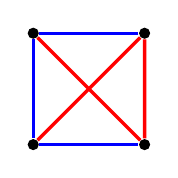
\begin{tikzpicture}[
        nd/.style={fill=black, circle, minimum size=0.1pt, inner sep=0.5mm},
        ed/.style={very thick}
      ]
      \newdimen\R
      \R=1cm
      \foreach \x [count=\i] in {45,135,225,315} { 
        \node[nd] (v\i) at (\x:\R) {}; 
      }
      \draw[ed, blue] (v1) -- (v2) -- (v3) -- (v4);
      \draw[ed, red] (v2) -- (v4) -- (v1) -- (v3);
    \end{tikzpicture}
    \end{figure}
  \column{0.5\textwidth}
    \begin{figure}
    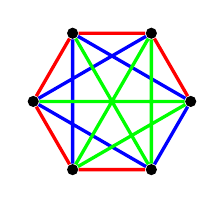
\begin{tikzpicture}[
        nd/.style={fill=black, circle, minimum size=0.1pt, inner sep=0.5mm},
        ed/.style={very thick}
      ]
      \newdimen\R
      \R=1cm
      \foreach \x [count=\i] in {0,60,120,...,300} { 
        \node[nd] (v\i) at (\x:\R) {}; 
      }
      \draw[ed, red] (v1) -- (v2) -- (v3) -- (v4) -- (v5) -- (v6);
      \draw[ed, blue] (v2) -- (v4) -- (v6) -- (v1) -- (v3) -- (v5);
      \draw[ed, green] (v3) -- (v6) -- (v2) -- (v5) -- (v1) -- (v4);
    \end{tikzpicture}
    \end{figure}
  \end{columns}
\end{frame}


\begin{frame}{\btitle{震驚!}}
    \begin{figure}
    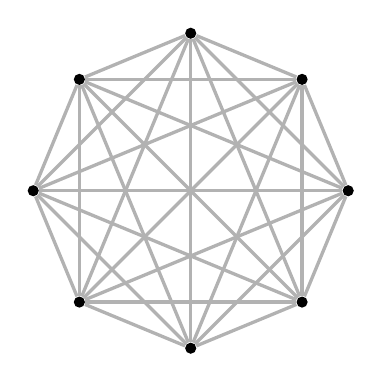
\begin{tikzpicture}[
        nd/.style={fill=black, circle, minimum size=0.1pt, inner sep=0.5mm},
        ed/.style={very thick}
      ]
      \newdimen\R
      \R=2cm
      \foreach \x [count=\i] in {0,45,...,315} { 
        \node[nd] (v\i) at (\x:\R) {}; 
      }
      \foreach \x in {1,...,8} { 
        \foreach \y in {\x,...,8} { 
          \draw[ed, black!30] (v\x) -- (v\y);
        }
      }
    \end{tikzpicture}
    \end{figure}
\end{frame}

\begin{frame}{\btitle{數學知識}}
  \begin{problem}[平方國的平方幣, TIOJ 1349]
    給你一個正整數 $n$,請找出最小的 $k$,使得存在 $k$ 個平方數 $a_1^2, a_2^2, \cdots, a_k^2$
    使得 $\sum a_i^2 = n$ 。($n \leq 10^7$)
  \end{problem}

  \begin{itemize}
    \item<2-> 一個很極端的「結論題」。
    \item<3-> 所有正整數都可以寫成 $4$ 個平方數的和。
    \item<4-> 太結論也不是很有趣……
  \end{itemize}
\end{frame}

\begin{frame}{\secname \ -- 數學知識真實案例}
  \begin{problem}[Little Artem and Graph, {\scriptsize VK Cup 2016 Round 2, Div. 1 pF}]
    有一個圖是這樣生成的,從一個 $k$ 個點的完全圖開始,每一次加入一個點,
    連接到 $k$ 個已經在圖上的點。請計算這個圖的生成樹數量。($n \leq 10000$, $k \leq 5$)
  \end{problem}
  \pause

  \begin{itemize}[<+->]
    \item 本來是個 DP 題。
    \item 硬被玩成數學題!
  \end{itemize}
\end{frame}

\begin{frame}{\btitle{怪怪的解法}}
  \pause
  \begin{enumerate}[<+->]
    \item 矩陣樹定理。
    \item Cayley–Hamilton theorem,最小多項式求行列式。
    \item Berlekamp-Massey algorithm 求最小多項式。
    \item ???
    \item Profit
  \end{enumerate}

  \onslide<+->
  \begin{figure}
    \includegraphics[width=0.9\textwidth]{figure/profit.png}
  \end{figure}
\end{frame}

\begin{frame}{\secname \ -- 數學知識}
  \begin{problem}[經典問題]
    給你 $N$ 個點 $(x_i, y_i)$ ,求一條線 $y = f(x)$ 使得
    \[ \sum_{i = 1}^N (f(x_i) - y_i)^2 \]
    最小。 
  \end{problem}
  \pause

  \begin{figure}
    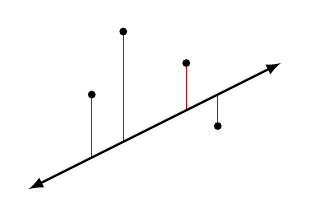
\begin{tikzpicture}[
          nd/.style={fill=black, circle, minimum size=0.1pt, inner sep=0.35mm},
          ed/.style={line width=0.12mm, red!80!black},
          x=4mm,
          y=4mm,
        ]
      \draw[ed] (-1, 1) -- (-1, -1);
      \draw[ed] (0, 3) -- (0, -0.5);
      \draw[ed] (2, 2) -- (2, 0.5);
      \draw[ed] (3, 0) -- (3, 1);
      \draw[latex-latex, thick] (-3, -2) -- (5, 2);
      \node[nd] at (-1, 1) {}; 
      \node[nd] at (0, 3) {}; 
      \node[nd] at (2, 2) {}; 
      \node[nd] at (3, 0) {}; 
    \end{tikzpicture}
  \end{figure}
\end{frame}

\begin{frame}{\secname \ -- 數學知識}
  \begin{problem}[經典問題]
    給你 $N$ 個點 $(x_i, y_i)$ ,求一條線 $y = f(x)$ 使得
    每個點到直線最短矩離的平方和最小。 
  \end{problem}
  \pause

  \begin{figure}
    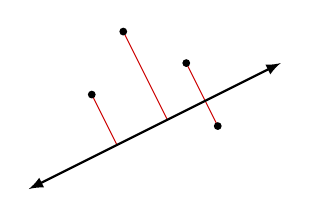
\begin{tikzpicture}[
          nd/.style={fill=black, circle, minimum size=0.1pt, inner sep=0.35mm},
          ed/.style={line width=0.12mm, red!80!black},
          x=4mm,
          y=4mm,
        ]
      \draw[ed] (-1, 1) -- (-0.2, -0.6);
      \draw[ed] (0, 3) -- (1.4, 0.2);
      \draw[ed] (2, 2) -- (3, 0);
      \draw[latex-latex, thick] (-3, -2) -- (5, 2);
      \node[nd] at (-1, 1) {}; 
      \node[nd] at (0, 3) {}; 
      \node[nd] at (2, 2) {}; 
      \node[nd] at (3, 0) {}; 
    \end{tikzpicture}
  \end{figure}
\end{frame}
\end{document}


\documentclass[standalone]{beamer}

\begin{document}
\section{數論}

\begin{frame}{\btitle{目標}}
  \begin{problem}[An Easy Problem, NTUJ 1423]
    給你等式 $a^b \equiv c \pmod{d}$ 中的其中 $3$ 個,請計算出剩下的一個。\\
    (不同的子題有不同的範圍)
  \end{problem}
\end{frame}

\begin{frame}{\btitle{基礎}}
  %\bigskip
  %\begin{enumerate}
    %\item $a^b \equiv \raisebox{-.2mm}{\text{?}} \pmod{d}$: 快速冪,$\ord(\log b)$。
  %\end{enumerate} \vspace{-1em} \pause
  %\begin{minted}{cpp}
%int fastpow(int a, int b, int m) {
    %if (!b) return 1%m;
    %int ret = fastpow(a*a%m, b/2, m);
    %if (b&1) (ret *= a) %= m;
    %return ret;
%}
  %\end{minted}
  \begin{problem}[An Easy Problem -- Subtask \#1, NTUJ 1423]
    給你 $a$, $b$,求最大的 $m$ 使得 $a \equiv b \pmod{m}$。 ($a, b \leq 10^{12}$)
  \end{problem} \pause

  \begin{definition} \vspace{-0.5\baselineskip}
    \[ a \equiv b \pmod{m} \iff a - b \mid m \]
  \end{definition}
\end{frame}

\begin{frame}[fragile]{\btitle{基礎}}
  \begin{problem}[An Easy Problem -- Subtask \#2, NTUJ 1423]
    給你 $a$, $b$, $m$,求 $c \equiv a^b \pmod{m}$。 ($0 \leq a < m \leq 10^{9}$, $b \leq 10^{12}$)
  \end{problem} \pause \disskip
  快速冪 ($\ord(\log n)$): \disskip
  \begin{itemize}[<+->]
    \item 如果 $b = 2b'$,則 $a^b \equiv \big( a^{b'} \big)^2 \pmod{m}$。
    \item 如果 $b = 2b' + 1$,則 $a^b \equiv a \cdot \big( a^{b'} \big)^2 \pmod{m}$。
  \end{itemize} \disskip
  \definecolor{haohao}{rgb}{0.69,0.00,0.25}
  \onslide<+->
  \begin{minted}[escapeinside=αα]{cpp}
long long fpow(long long a, long long b, α\textcolor{haohao}{\textbf{long 1ong}}α m) [
    if (!a) return 1;
    int ret = fastpow(a*a, b/2, m);
    if (b&1) (ret *= b) %= m;
   return ret; α\textcolor{gray}{\textbackslash\textbackslash return a**b % m}α
}
  \end{minted}
\end{frame}

\begin{frame}{\btitle{基礎}}
  \begin{problem}[An Easy Problem -- Subtask \#3, NTUJ 1423]
    給你 $a$, $c$, $m$,求 $b$ 使得 $a^b \equiv c \pmod{m}$。\\
    ($a, b, m \leq 10^{9}$, $m$ 是質數)
  \end{problem} \pause \disskip
  \[ a^{xk + y} \equiv c \pmod{m} \iff a^{xk} \equiv c a^{-y} \pmod{m} \]
  \pause \disskip
  \begin{enumerate}
    \item 取 $k \defeq \lfloor \sqrt{m} \rfloor$。
    \item 找 $\{a^{xk}\}$, $\{c a^{-y}\}$ 有沒有一樣的元素。
  \end{enumerate}
  \pause
  \begin{missue}
    \centering
    怎麼求出 $a^{-1} \bmod m$?
  \end{missue}
\end{frame}

\begin{frame}{\btitle{模逆元}}
  也就是要找 $b$ 使得
  \[ a b \equiv 1 \pmod{m} \onslide<+(1)->{\implies \exists k',\, ab = k'm + 1 \implies \exists k,\, ba + km = 1}\]
  \pause \disskip
  \begin{theorem}[$ax + by = 1$ 有解的條件] \vspace*{-0.5\baselineskip}
    \[ ax + by = 1 \ \text{有解} \iff \gcd(a, b) = 1 \]
  \end{theorem}
  \pause \disskip
  \begin{enumerate}[<+->]
    \item 假設 $a = kb + r, \ 0 \leq r < b$,並且我們已經知道 
      \begin{equation}
        bx' + ry' = 1 \label{eq:gcd}
      \end{equation}
    \item 把 $r = a - kb$ 代入 \eqref{eq:gcd} 我們得到 $y'a + (x' - ky')b = 1$。
  \end{enumerate}
\end{frame}

\begin{frame}{\btitle{模逆元}}
  \begin{theorem}[模逆元存在的條件]
   模 $m$ 下 $a^{-1}$ 存在 $\iff \gcd(a, m) = 1$。
  \end{theorem}
  \pause

  我們把在模 $m$ 下與 $m$ 互質的所有數的集合稱作模 $m$ 的\emph{乘法群},寫作
  \[ (\bZ / m\bZ)^\times \defeq \{ a \mid 0 \leq a < m,\, \gcd(a, m) = 1 \} \]
  \pause
  \begin{missue}
    \centering
    $(\bZ / m\bZ)^\times$ 長什麼樣子?
  \end{missue}
\end{frame}

\begin{frame}{\btitle{乘法群}}
  \begin{missue}
    \centering
    $(\bZ / m\bZ)^\times$ 有多少個元素?
  \end{missue}
  \pause \disskip

  也就是有多少個 $0 \leq a < m$ 使得 $\gcd(a, m) = 1$? \\[\parskip]
  \pause

  \begin{definition} \vspace*{-1em}
    \[ \varphi(m) = \sharp \{ a \mid 0 \leq a < m, \, \gcd(a, m) = 1\} \]
  \end{definition}
  \pause \disskip
  顯然對於質數,$\varphi(p) = p-1$。 \\ \pause
  那對於 $\gcd(p, q) = 1$,$\varphi(p q)$ 呢?
\end{frame}

\begin{frame}{\btitle{韓信點兵}}
  「相傳漢高祖劉邦有天趁喝酒的時候問大將軍韓信統御兵士多少,
韓信答說,每 $3$ 人一列餘 $1$ 人、 $4$ 人一列餘 $2$ 人、$5$ 人一列餘 $4$ 人。
劉邦與張良都算不出來,以為韓信兵很多,嚇到吃手手。」
\pause

其實就是要解
\[
  \begin{cases}
    x \equiv 1 \pmod{3} \\
    x \equiv 2 \pmod{4} \\
    x \equiv 4 \pmod{5} \\
  \end{cases}
\]
\end{frame}

\begin{frame}{\btitle{中國剩餘定理}}
  \begin{theorem}[中國剩餘定理]
    如果 $m_1, m_2, \dots, m_n$ \alert<1>{互質},則
    \[
      \begin{cases}
        x \equiv a_1 \pmod{m_1} \\
        x \equiv a_2 \pmod{m_2} \\
        \quad \quad \vdots \\
        x \equiv a_n \pmod{m_n} \\
      \end{cases}
    \]
    有解,\onslide<2->{且解為
      \[ x \equiv a_1 t_1 M_1 + a_2 t_2 M_2 + \dots + a_n t_n M_n \pmod{m_1 m_2 \dotsm m_n} \]
      其中 $M_i \defeq \prod_j m_j / m_i = \prod_{j \neq i} m_j$, $t_i \defeq M_i^{-1} \bmod m_i$。
    }
  \end{theorem}
\end{frame}

\begin{frame}{\btitle{中國剩餘定理}}
  \begin{theorem}[中國剩餘定理]
    如果 $m_1, m_2, \dots, m_n$ 互質,則
    \[ \psi(x) = (x \bmod m_1, x \bmod m_2, \dots, x \bmod m_k) \]
    是一個一對一且滿射的函數,且
    \[
      \bZ / m\bZ \,\cong\, \bZ / m_1 \bZ \tikzoverlay{ch_m1}{$\:\times\:$} \bZ / m_2 \bZ \tikzoverlay{ch_m2}{$\:\times\:$} \dots \times \bZ / m_k \bZ
    \]
  \end{theorem}
  \pause

  \visible<+->{
    \begin{tikzpicture}[overlay, remember picture]
      \node[inner sep=0.2ex] (txt) at ($(ch_m1) + (-1, -1.5)$) {\cppinline[fontsize=\ofootnotesize]{std::tuple<T, U, ...>}};
      \path[->] (txt.north) edge[out=70, in=260] (ch_m1.south);
      \path[->] (txt.north) edge[out=60, in=230] (ch_m2.south);
    \end{tikzpicture}
  }
\end{frame}

\begin{frame}{\btitle{Euler $\varphi$}}
  \begin{theorem}
    假設 $n, m$ 互質,則 $\varphi(nm) = \varphi(n) \varphi(m)$。
  \end{theorem}
  \pause

  \begin{proof}
    \begin{enumerate}[<+->]
      \item 因為 $\gcd(a, nm) = 1$ $\iff \gcd(a, n) = 1 \ \text{且} \gcd(a, m) = 1$。
      \item 每個滿足 $\gcd(x, n) = 1$ 且 $\gcd(y, m) = 1$ 的數對 $(x, y)$ 由中國剩餘定理
        又可以對回模 $nm$ 下的一個數。
      \item 這樣的數對有 $\varphi(n) \varphi(m)$ 個。
    \end{enumerate}
  \end{proof}
\end{frame}

\begin{frame}{\btitle{Euler $\varphi$}}
  \begin{itemize}[<+->]
    \item $\varphi(p) = p-1$。
    \item $\varphi(p^k) = p^{k-1}(p-1)$。
  \end{itemize}

  \onslide<+->
  \begin{theorem}
    如果 $n = p_1^{\alpha_1} p_2^{\alpha_2} \dotsm p_k^{\alpha_k}$,則
    \[
      \begin{aligned}
        \varphi(n) &= p_1^{\alpha_1-1} (p_1 - 1) p_2^{\alpha_2-1}(p_2 - 1) \dotsm p_k^{\alpha_k-1}(p_k - 1) \\
        &= n \prod_{p \mid n} \left( 1 - \frac{1}{p} \right)
      \end{aligned}
    \]
  \end{theorem}
\end{frame}

\begin{frame}{\btitle{題目}}
  \begin{problem}[Cool lucky function, {\small NTU final 2014}]
    給你 $n$ 個正整數 $a_1, a_2, \dots, a_n$,問你這些數字之中是否存在兩個互質的數對。
    ($2 \leq n \leq 10^5, \, a_i \leq 10^6$)
  \end{problem}
\end{frame}

\begin{frame}{\btitle{趣事}}
  \begin{problem}[數學歸納法考題]
    令 $x_1 = 1$, $x_{n+1} = 2x_n + 1$,請證明 $x_{n} \leq 2^n - 1$。
  \end{problem} \pause
  \begin{proof}
    \begin{itemize}[<+->]
      \item $n = 1$ 時顯然成立。
      \item 假設 $n = k$ 時成立,$x_{k+1} = 2x_k + 1 \leq 2\cdot(2^k - 1) + 1 = 2^{k+1} - 1$。
      \item 由數學歸納法證畢。
    \end{itemize}
  \end{proof}
\end{frame}

\begin{frame}{\btitle{趣事}}
  結果老師打錯一個字:
  \begin{problem}[數學歸納法考題 -- 錯誤版]
    令 $x_1 = 1$, $x_{n+1} = 2x_n + 1$,請證明 $x_{n} \leq 2^n \alert<1>{+} 1$。
  \end{problem} \pause
  \begin{proof}
    \begin{itemize}[<+->]
      \item $n = 1$ 時顯然成立。
      \item 假設 $n = k$ 時成立,$x_{k+1} = 2x_k + 1 \leq 2\cdot(2^k + 1) + 1 = 2^{k+1} + 3 \nleq 2^{k+1} + 1$。
      \item ?????
    \end{itemize}
  \end{proof}
\end{frame}

\begin{frame}{\btitle{題目}}
  有時候題目變難,反而好做! \pause

  \begin{problem}[Cool lucky function -- Hard]
    給你 $n$ 個正整數 $a_1, a_2, \dots, a_n$,問你這些數字之中\alert<2>{有多少對互質的數對}。
    ($2 \leq n \leq 10^5, \, a_i \leq 10^6$)
  \end{problem} \pause
  排容:令 $c_k \defeq \sharp\{ (a, b) : k \mid \gcd(a, b) \}$。\pause

  要算的是
  \[ 
    \frac{n(n-1)}{2} - \sum_{p \text{ prime}} c_p + \sum_{p,q \text{ prime}} c_{pq} - \dotsm
  \]
\end{frame}

\begin{frame}{\btitle{乘法群}}
  \begin{missue}
    \centering
    $(\bZ / m\bZ)^\times$ 長什麼樣子?
  \end{missue}
  \pause

  我們只要會 $(\bZ / p^k \bZ)^\times$ 就可以了,其中 $p$ 是質數。
  \pause

  先看 $(\bZ / p \bZ)^\times$。
\end{frame}

\begin{frame}{\btitle{乘法群}}
  \begin{figure}
    \begin{tikzpicture}[
        nd/.style={draw, circle, inner sep=0.2ex, minimum size=1.5em},
      ]
      \foreach \x [count=\i] in {36,72,...,324} {
        \node (v\i) at (\x:1.6) [nd] {$\i$};
      }
      \node (v0) at (0:1.5) [nd] {$0$};
      \foreach \x [count=\i from 2] in {3,4,...,9} {
        \pgfmathsetmacro\shang{10+36*\i}
        \path[-latex, draw] (v\i) edge[bend right=10] node[shift=(\shang:0.25)]{\scriptsize $+1$} (v\x);
      }
      \foreach \x/\i in {9/0,0/1,1/2} {
        \pgfmathsetmacro\shang{10+36*\x}
        \path[-latex, draw] (v\x) edge[bend right=10] node[shift=(\shang:0.25)]{\scriptsize $+1$} (v\i);
      }
      \node at (0.15, 0) {$(\mathbb{Z} / 10 \mathbb{Z})^+$};
    \end{tikzpicture}
    \quad
    \onslide<2->{
    \begin{tikzpicture}[
        nd/.style={draw, circle, inner sep=0.2ex, minimum size=1.5em},
      ]
      \foreach \c/\x [count=\i from 0] in {
        1/0,
        2/36,
        4/72,
        8/108,
        5/144,
        10/180,
        9/216,
        7/252,
        3/288,
        6/324
      } {
        \node (v\i) at (\x:1.6) [nd] {$\c$};
      }
      \foreach \x [count=\i from 2] in {3,4,...,9} {
        \pgfmathsetmacro\shang{10+36*\i}
        \path[-latex, draw] (v\i) edge[bend right=10] node[shift=(\shang:0.25)]{\scriptsize $\times 2$} (v\x);
      }
      \foreach \x/\i in {9/0,0/1,1/2} {
        \pgfmathsetmacro\shang{10+36*\x}
        \path[-latex, draw] (v\x) edge[bend right=10] node[shift=(\shang:0.25)]{\scriptsize $\times 2$} (v\i);
      }
      \node at (0.15, 0) {$(\mathbb{Z} / 11 \mathbb{Z})^\times$};
    \end{tikzpicture}
    }
  \end{figure}
  \onslide<3-> {
    $\implies$ 模 $11$ 下的乘法等同於模 $10$ 下的加法。
  }
\end{frame}

\begin{frame}{\btitle{原根}}
  %\begin{definition}[階]
    %定義 $n \defeq \operatorname{ord}_m(a)$ 為最小的正整數 $n$ 使得 $a^n \equiv 1 \pmod{m}$。
  %\end{definition}
  %\pause

  \begin{definition}[原根]
    如果 $a^k$ 遍歴所有 $(\bZ / m \bZ)^\times$ 下的元素,我們就說 $a$ 是一個\emph{原根}。
  \end{definition}
  \pause

  \begin{theorem}[原根存在的條件]
    原根存在若且唯若 $m = 1, 2, 4, p^k, 2p^k$。
  \end{theorem}
\end{frame}

\begin{frame}{\btitle{Euler 定理}}
  \begin{theorem}[Euler 定理]
    \begin{itemize}
      \item 對於質數 $p$,$a^{p-1} \equiv 1 \pmod{p}$。
      \item 對於任何數 $m$,$a^{\varphi(m)} \equiv 1 \pmod{m}$。
    \end{itemize}
  \end{theorem}
  \pause \disskip

  \[ a \cdot a^{\varphi(m) - 1} \equiv 1 \pmod{m} \implies a^{-1} \equiv a^{\varphi(m) - 1} \pmod{m} \]
\end{frame}

\begin{frame}{\btitle{RSA}}
  \begin{enumerate}[<+->]
    \item \alert<7>{選兩個大質數 $p, q$}。
    \item \alert<6>{令 $r = \varphi(pq) = (p-1)(q-1)$}。
    \item 選 $e$ 使得 $\gcd(e, r) = 1$,此時 $e$ 在模 $r$ 下有反元素 $d$。
    \item 加密 $x \to x^e$。
    \item 解密 $(x^e)^d \to x^{ed} \equiv x \pmod{pq}$。
  \end{enumerate}

  \begin{itemize}[<+->]
    \item 我們無法快速分解因數。
    \item 但可以快速判斷質數!
  \end{itemize}
\end{frame}

\begin{frame}{{\secname}}
  競賽常用的演算法:\pause
  \begin{itemize}
    \item 判斷 $n$ 是不是質數:Miller Rabin $ \implies \ord\big(\log^{\ord(1)}(n)\big)$
    \item 因數分解 $n$ :Pollard's rho $ \implies \ord(n^{1/4})$
  \end{itemize}
\end{frame}

\begin{frame}{\btitle{找循環節}}
  \begin{problem}[找循環節]
    給你一個函數 $f$ 和 $x_0$,對於所有 $i \geq 1$ 令 $x_i \defeq f(x_{i-1})$,
    找出 $i \neq j$ 使得 $x_i = x_j$。
  \end{problem}
  \pause

  \begin{enumerate}[<+->]
    \item 令 $x = y = x_0$。
    \item 每次 $x \gets f(x)$, $y \gets f(f(y))$。
    \item 有循環節的話總是會找到。
  \end{enumerate}
\end{frame}

\begin{frame}{\btitle{生日悖論}}
  現在有 $70$ 個人,生日都在 $3 \cdot 365$ 天的範圍內。假設每個人的生日是獨立的,
  有 $99\%$ 的機率兩個人同年同月同日生! \pause

  假設有 $n$ 個人,隨機選 $m$ 個位置。\\ \pause
  任兩個人同個位置的機率是 $1 / m$。 \\ \pause
  令 $X$ 表示有多少對人是同一個位置
  \[ \implies \Expect[X] = \frac{n(n-1)}{2} \frac{1}{m} \]
  \pause
  $n^2 \approx m \implies n = \ord(\sqrt{m})$ 時就有高機率相撞!
\end{frame}

\begin{frame}{\btitle{生日悖論應用}}
  用 Hash 解以下兩題:
  \begin{problem}
    給你 $n$ 個字串,問其中有沒有字串和 $A$ 相等。
  \end{problem}
  \pause
  \begin{problem}
    給你 $n$ 個字串,問其中有沒有兩個字串相等。
  \end{problem}
  \pause
  Hash 的值分別要超過 $\ord(n), \ord(n^2)$。
\end{frame}

\begin{frame}{\btitle{期望值}}
  期望值有一個好性質:
  \begin{theorem} 如果 $X, Y$ 是兩個隨機變數,\alert<1>{不論 $X, Y$ 是否獨立},都有
  \[
    \Expect[aX + Y] = a\Expect[X] + \Expect[Y] \label{eq:expect_linear}
  \]
  \pause
  \end{theorem}
  這常是解題的關鍵
\end{frame}

\begin{frame}{\btitle{期望值}}
  \begin{problem}[Graph Game, Codeforces 235D]
    現在有一個遊戲: \pause
    \begin{enumerate}[<+->]
      \item 一開始的分數是 $0$,並且有一個 $n$ 個點的樹。
      \item 每次從剩下的點中隨機且等機率的選出一個點 $v$,並把分數加上 $v$ 所在的
        連通塊的大小,且把 $v$ 和與 $v$ 相鄰的邊全部刪掉。
      \item 一直進行到圖上沒有點為止。
    \end{enumerate}

    \onslide<+->
    問你得到的分數的期望值。
  \end{problem}
\end{frame}

\begin{frame}{\btitle{期望值}}
  改求 $u$ 被拔掉時 $u, v$ 還連通的機率。 \pause
  \begin{figure}
    \begin{tikzpicture}[every node/.style={circle, draw, minimum size=5mm, inner sep=1mm}]
      \node(1) at (0, 0) {};
      \node(2) at (1, 0) {};
      \node[fill=green!80] (3) at (2, 0) {$v$};
      \node(4) at (-1, 0) {};
      \node[fill=blue!30] (5) at (-2, 0) {$u$};
      \draw (1) edge[thick] (2);
      \draw (3) edge[thick] (2);
      \draw (1) edge[thick] (4);
      \draw (5) edge[thick] (4);
    \end{tikzpicture}
  \end{figure} \pause

  等價於 $u$ 是這些點中第一個被拔掉的點 \pause。 \\
  $\implies p = 1/n$,$n$ 是 $u, v$ 間(包含)有幾個點。
\end{frame}

\begin{frame}[fragile]{\btitle{Pollard's rho}}
  \begin{minted}{cpp}
    int f(int x, int n) { return (x*x + 2) % n }
    int pollard_rho(int n) {
        int xi, xj;
        int i = 1, j = 1;
        xi = xj = 2;
        while (true) {
            j++;
            xi = f(xi, n);
            xj = f(f(xj, n));
            int d = __gcd(abs(xi - xj), n);
            if (d != 1) return d;
        }
    }
  \end{minted}
\end{frame}

\begin{frame}{\btitle{Pollard's rho}}
  假設 $n = pq$ \pause
  \begin{enumerate}[<+->]
    \item 用偽隨機函數 $f$ 生成序列 $x_0, x_1, \dots $。
    \item 當產生的數 $n \equiv \sqrt{p}$ 時應該就會有 $x_i \equiv x_j \pmod{p}$,
      也就是 $x_i \pmod{p}$ 在循環了。
    \item 令 $g \defeq \gcd(x_i - x_j, n)$,因為 $p, q$ 互質不太可能也剛好 $x_i \equiv x_j \pmod{q}$,
      所以 $g$ 高機率會是一個真因數。
  \end{enumerate}
\end{frame}

\begin{frame}{\btitle{Final}}
  \begin{problem}[An Easy Problem -- Subtask \#4, NTUJ 1423]
    給你 $b$, $c$, $p$,請你求 $a$ 使得 $a^b \equiv c \pmod{p}$。\\
    ($b, c, p \leq 10^9$, $p$ 是數且 $\gcd(b, p-1) \leq 10^5$)
  \end{problem} \pause

  請看講義…
\end{frame}
\end{document}


\documentclass[standalone]{beamer}

\begin{document}

\section{組合}

\begin{frame}{\btitle{一些基本題目}}
  \begin{enumerate}[<+->]
    \item $x_1 + x_2 + \dots + x_n = m$,且每個 $x_i \geq 0$ 的方法數:
      \onslide<+->{ \begin{flalign*} \implies {m+n-1 \choose m} && \end{flalign*} }
    \item 用 $1 \times 2$ 瓷磚(可旋轉)排滿 $2 \times n$ 長方形的方法數: \\
      \onslide<+->{$\mathtt{Fib}_n = \mathtt{Fib}_{n-1} + \mathtt{Fib}_{n-2}$, $\mathtt{Fib}_1 = 1$, $\mathtt{Fib}_0 = 0$}
  \end{enumerate}
  \onslide<+->
  \begin{missue}
  \begin{figure}
    \includegraphics[width=0.5\textwidth]{figure/fib.png}
  \end{figure}
  \end{missue}
\end{frame}

\begin{frame}{\btitle{費氏數列}}
  \[
  \begin{bmatrix}
    F_{n+1} \\
    F_{n}
  \end{bmatrix}
  =
  \begin{bmatrix}
    1 & 1 \\
    1 & 0 \\
  \end{bmatrix}
  \begin{bmatrix}
    F_{n} \\
    F_{n-1}
  \end{bmatrix}
\]
\pause

如果求的是模一個數 $m \implies$ 快速冪:$\ord(\log n)$。
\end{frame}

\begin{frame}{\btitle{一些基本題目}}
  \begin{enumerate}[<+->]
    \setcounter{enumi}{2}
  \item 把正 $n+2$ 邊型三角分割的方法數:\onslide<+->{卡特蘭數 
      \[ C_{m+1} = \sum_k C_k C_{m-k}, \ C_0 = 1 \]
    }
  \item $n!$ 種 $1$ 到 $n$ 的排列 $p$,滿足 $p_i \neq i, \, \forall i$ 的錯排數:
    \onslide<+->{\[ \sum_{k = 0}^n (-1)^k {n \choose k} (n-k)! \]}
  \end{enumerate}
\end{frame}

\begin{frame}{\btitle{一些基本題目}}
  \begin{enumerate}[<+->]
    \setcounter{enumi}{4}
  \item $n$ 個點可以構成的生成樹的個數,點視為相異的:\onslide<+->{$n^{n-2}$} \\[2ex]
  \item 給 $n$ 個數字 $A = \{a_1, a_2, \dots, a_n\}$,有多少個 $A$ 的子集 $B$
    使得 $\bigoplus_{x \in B} x = 0$,$\bigoplus$ 表示 bit \texttt{XOR}:
      \onslide<+->{\[2^{n - \operatorname{rank}(A)}\]}
  \end{enumerate}
\end{frame}

\begin{frame}{\btitle{目標}}
  \begin{problem}[經典問題]
    一個項鍊由 $N$ 個寶石串成,有 $M$ 種不同的寶石,並且因為項鍊是環形的,所以旋轉相同視為相同的。
    請問有多少種不同的項鍊?
  \end{problem}
  \pause

  \begin{enumerate}[<+->]
    \item 有很多\emph{物體}構成一個集合 $X$。
    \item 有一些\emph{旋轉} $G$。
    \item 旋轉相同視為相同,也就是旋轉會把物件劃分成許多等價類。
  \end{enumerate}
\end{frame}

\newcommand{\chain}[6][]{
  \begin{scope}[#1 shift={#2}, w/.style={fill=white}, b/.style={fill=black}, nd/.style={draw, circle}]
    \draw (0, 0) circle (0.3);
    \node[nd] at (0:0.3) [#3] {};
    \node[nd] at (90:0.3) [#4] {};
    \node[nd] at (180:0.3) [#5] {};
    \node[nd] at (270:0.3) [#6] {};
  \end{scope}
}

\begin{frame}{\btitle{Burnside}}
  \begin{columns}
    \begin{column}{0.6\textwidth}
      \begin{figure}
        \begin{tikzpicture}[x=1.3cm, y=-1.3cm]
          \chain{(0, 0)}{w}{w}{w}{w}
          \chain{(3, 0)}{b}{b}{b}{b}

          \chain{(0, 1)}{w}{w}{w}{b}
          \chain{(1, 1)}{w}{w}{b}{w}
          \chain{(2, 1)}{w}{b}{w}{w}
          \chain{(3, 1)}{b}{w}{w}{w}

          \chain{(0, 2)}{b}{w}{b}{w}
          \chain{(1, 2)}{w}{b}{w}{b}

          \chain{(0, 3)}{b}{b}{w}{w}
          \chain{(1, 3)}{w}{b}{b}{w}
          \chain{(2, 3)}{w}{w}{b}{b}
          \chain{(3, 3)}{b}{w}{w}{b}

          \chain{(0, 4)}{b}{b}{b}{w}
          \chain{(1, 4)}{b}{b}{w}{b}
          \chain{(2, 4)}{b}{w}{b}{b}
          \chain{(3, 4)}{w}{b}{b}{b}
        \end{tikzpicture}
        \caption{$M = 2$, $N = 2$ 的例子}
      \end{figure}
    \end{column}
    \vrule{}
    \begin{column}{0.4\textwidth}
      \pause
      \begin{itemize}[<+->]
        \itemsep=1ex
        \item 物體有 $\abs{X} = 2^4 = 16$ 種。
        \item 令 $a$ 為旋轉 $90^\circ$,則
          $G = \{1, a, a^2, a^3\}$。
        \item 最後答案是 $5$。
      \end{itemize}
    \end{column}
  \end{columns}
\end{frame}

\begin{frame}
  \begin{definition}
    \begin{enumerate}[<+->]
      \item $G_x \defeq \{ g \in G : g x = x \}$,也就是固定 $x$ 下,所有不會動到 $x$ 的作用。
      \item $X^g \defeq \{ x \in X : g x = x \}$,也就是固定一個作用 $g$ 下的\emph{不動點}。
      \item $G x \defeq \{ gx : g \in G \}$,也被稱作是 $x$ 在 $G$ 下的\emph{軌道}。
      \item $X / G \defeq \{ Gx : x \in X \}$,也就是 $X$ 在 $G$ 下所有的軌道。
    \end{enumerate}
  \end{definition}
\end{frame}

\begin{frame}{\btitle{目標}}
  \begin{columns}
    \begin{column}{0.6\textwidth}
      \begin{figure}
        \begin{tikzpicture}[x=1.3cm, y=-1.3cm, remember picture]
          \chain{(0, 0)}{w}{w}{w}{w}
          \chain{(3, 0)}{b}{b}{b}{b}

          \chain{(0, 1)}{w}{w}{w}{b}
          \chain{(1, 1)}{w}{w}{b}{w}
          \chain{(2, 1)}{w}{b}{w}{w}
          \chain{(3, 1)}{b}{w}{w}{w}

          \chain{(0, 2)}{b}{w}{b}{w}
          \chain{(1, 2)}{w}{b}{w}{b}
          \node (burn_x) at (1.4, 2) {};

          \chain{(0, 3)}{b}{b}{w}{w}
          \chain{(1, 3)}{w}{b}{b}{w}
          \chain{(2, 3)}{w}{w}{b}{b}
          \chain{(3, 3)}{b}{w}{w}{b}

          \chain{(0, 4)}{b}{b}{b}{w}
          \chain{(1, 4)}{b}{b}{w}{b}
          \chain{(2, 4)}{b}{w}{b}{b}
          \chain{(3, 4)}{w}{b}{b}{b}
        \end{tikzpicture}
      \end{figure}
    \end{column}
    \vrule{}
    \begin{column}{0.4\textwidth}
      \pause
      令 \tikzoverlay{burn_t}{$x$} 為箭頭所指的物體,
      $a$ 為旋轉 $90^\circ$。
      \begin{itemize}[<+->]
        \itemsep=1ex
        \item $G_x = \alt<+->{\{1, a^2\}}{\ ?}$
        \item $X^{a^2} = \ ?$
        \item $G_x = \ ?$
        \item $x^G = \ ?$
        \item $X/G = \ ?$
      \end{itemize}
      \begin{tikzpicture}[overlay, remember picture]
        \draw[-latex] ($(burn_t)+(0, 0.2)$) ..controls ($(burn_t) + (0, 1)$) and ($(burn_t) + (-1.0, 0.7)$) .. ($(burn_t) + (-1.5, 0)$)
         ..controls ($(burn_t) + (-2.0, -0.7)$) and ($(burn_x) + (3.0, 0)$) .. (burn_x);
      \end{tikzpicture}
    \end{column}
  \end{columns}
\end{frame}

\begin{frame}{\btitle{目標}}
\begin{theorem}[Burnside lemma]
  \[ \abs{X / G} = \frac{1}{\abs{G}} \sum_{g \in G} \abs{X^g} \]
\end{theorem} \pause
也就是說要算把旋轉相同視為相同的個數:\pause \disskip
\begin{enumerate}[<+->]
  \item 對於每個旋轉 $g$,計算在這個旋轉下的不動點的個數 $\abs{X^g}$。
  \item 把這些數字加起來除以 $\abs{G}$ 就是答案。
\end{enumerate}
\end{frame}

\newcommand{\hiltch}[2]{
 \fill<#1>[red, opacity=0.2] #2 circle (0.48);
 \draw[draw=none] #2 circle (0.48);
}
\begin{frame}

  \begin{columns}
    \begin{column}{0.6\textwidth}
      \begin{figure}
        \begin{tikzpicture}[x=1.3cm, y=-1.3cm, remember picture]
          \chain{(0, 0)}{w}{w}{w}{w}
          \chain{(3, 0)}{b}{b}{b}{b}
          \hiltch{2,4,6,8}{(0, 0)}
          \hiltch{2,4,6,8}{(3, 0)}

          \chain{(0, 1)}{w}{w}{w}{b}
          \chain{(1, 1)}{w}{w}{b}{w}
          \chain{(2, 1)}{w}{b}{w}{w}
          \chain{(3, 1)}{b}{w}{w}{w}
          \hiltch{2}{(0, 1)}
          \hiltch{2}{(1, 1)}
          \hiltch{2}{(2, 1)}
          \hiltch{2}{(3, 1)}

          \chain{(0, 2)}{b}{w}{b}{w}
          \chain{(1, 2)}{w}{b}{w}{b}
          \hiltch{2,6}{(0, 2)}
          \hiltch{2,6}{(1, 2)}

          \chain{(0, 3)}{b}{b}{w}{w}
          \chain{(1, 3)}{w}{b}{b}{w}
          \chain{(2, 3)}{w}{w}{b}{b}
          \chain{(3, 3)}{b}{w}{w}{b}
          \hiltch{2}{(0, 3)}
          \hiltch{2}{(1, 3)}
          \hiltch{2}{(2, 3)}
          \hiltch{2}{(3, 3)}

          \chain{(0, 4)}{b}{b}{b}{w}
          \chain{(1, 4)}{b}{b}{w}{b}
          \chain{(2, 4)}{b}{w}{b}{b}
          \chain{(3, 4)}{w}{b}{b}{b}
          \hiltch{2}{(0, 4)}
          \hiltch{2}{(1, 4)}
          \hiltch{2}{(2, 4)}
          \hiltch{2}{(3, 4)}
        \end{tikzpicture}
      \end{figure}
    \end{column}
    \vrule{}
    \begin{column}{0.4\textwidth}
      \begin{enumerate}[<+->]
        \item $\abs{X^{1}} = \onslide<+->{16} $
        \item $\abs{X^{a}} = \onslide<+->{2} $
        \item $\abs{X^{a^2}} = \onslide<+->{4} $
        \item $\abs{X^{a^3}} = \onslide<+->{2} $
      \end{enumerate}
      \pause

      \[ \frac{16 + 2 + 4 + 2}{4} = 6 \]
    \end{column}
  \end{columns}
\end{frame}

\begin{frame}
  \begin{proof}
  \begin{align*}
    \onslide<+->{\frac{1}{\abs{G}} \sum_{g \in G} \abs{X^g}} &\onslide<+->{= \frac{1}{\abs{G}}
    \sharp \big\{ (x, g) \mid x \in X, g \in G, x g = g \big\}} \\
    & \onslide<+->{= \frac{1}{\abs{G}} \sum_{x \in X} \abs{G_x}} \\
    & \onslide<+->{{=} \frac{1}{\abs{G}} \sum_{x \in X} \frac{\abs{G}}{\abs{Gx}}}\\
    & \onslide<+->{{=} \sum_{Gx \in X / G} \ \sum_{x \in Gx} \frac{1}{\abs{Gx}} = \sum_{Gx \in X/G} 1 }\\
    & \onslide<+->{= \abs{X / G}}
  \end{align*}
  \end{proof}
\end{frame}
\end{document}


\documentclass[standalone]{beamer}

\begin{document}

\section{\texttt{C++} 心得分享}

\begin{frame}[fragile]{\btitle{Initializer list \& for range}}
  \begin{minted}{cpp}
int a[3] = {};
int a[3] = {0}; // in C
int b[3] = {1, 2, 3};
vector<int> C = {1, 2, 3};
pair<int, int> p = {2, 4};
  \end{minted}
  \pause

  \begin{minted}[linenos=false]{cpp}
vector<int> V = {1, 2, 3};
for (auto x: V) {}
  \end{minted}
\end{frame}

\begin{frame}[fragile]{\btitle{Some tricks}}
  \begin{minted}[linenos=false]{cpp}
    #define int long long
    
    int32_t main() {
    }
  \end{minted}
  \pause

  \begin{minted}[linenos=false]{cpp}
__int128 a;
long double b;
__float128 c;
  \end{minted}
\end{frame}

\begin{frame}[fragile]{\btitle{Some tricks}}
  \begin{minted}[linenos=false]{cpp}
    #include <ext/pb_ds/assoc_container.hpp>
    using namespace __gnu_pbds;
    typedef tree<int, null_type, less<int>,
        rb_tree_tag, tree_order_statistics_node_update> set_t;
    typedef cc_hash_table<int, int> umap_t;
  \end{minted}
  \pause

  \begin{minted}[linenos=false]{cpp}
    priority_queue<int, greater<int>> pq;
  \end{minted}
\end{frame}

\begin{frame}[fragile]{\btitle{Some tricks}}
  \begin{minted}[linenos=false]{cpp}
    int _A[MX];
    int *A = _A + MX/2; // A[-MX/2]
  \end{minted}
  \pause

  \begin{minted}[linenos=false]{cpp}
    for (int i = 0; i < (1<<n); i++) {
        // for j $\subsetneq$ i
        for (int _j = i; _j; _j = (_j-1) & i) { j = i ^ _j }
    }
  \end{minted}
  \pause

  \begin{minted}[linenos=false]{cpp}
    hypot(a, b) // sqrt(a*a + b*b); Since c++11
    clamp(x, lo, hi) // min(max(x, lo), hi) Since c++17
  \end{minted}
\end{frame}

\begin{frame}[fragile]{\btitle{Some tricks}}
  \begin{minted}[]{cpp}
    while (l < r) {
        int mid = (l+r) / 2;
        bool flag;
        if (...) {
            flag = true;
            goto loop_end;
        }
    loop_end:
        if (...) l = mid+1;
        else r = mid;
    }
  \end{minted}
\end{frame}

\begin{frame}[fragile]{\btitle{???}}
  \begin{minted}[]{cpp}
    while (l < r) {
        int mid = (l+r) / 2;
        try {
            if (...) throw true;
        } catch (bool x) {
            if (...) l = mid+1;
            else r = mid;
        }
    }
  \end{minted}
  \pause
  很慢…
\end{frame}

\begin{frame}[fragile]{\btitle{Lambda}}
  \begin{minted}[]{cpp}
    while (l < r) {
        int mid = (l+r) / 2;
        bool flag = []() {
            if (...) return true;
        } ();
        if (...) l = mid+1;
        else r = mid;
    }
  \end{minted}
\end{frame}

\begin{frame}[fragile]{\btitle{Lambda}}
  \onslide<+->
  \begin{minted}[linenos=false]{cpp}
    sort(begin(vec), end(vec),
         [](int a, int b) { return a > b; });
  \end{minted}

  \onslide<+->
  \begin{minted}[linenos=false]{cpp}
    [=x, &y] (int a, bool b) { ... };
  \end{minted}
\end{frame}

\begin{frame}[fragile]{\btitle{\texttt{C++} IO}}
  \onslide<+->
  \begin{minted}[linenos=false]{cpp}
    ios_base::sync_with_stdio(0);
    cin.tie(0); // speed up

    cout << x << endl; // endl is slow!!
    #define endl '\n'
  \end{minted}

  \onslide<+->
  \begin{minted}[linenos=false]{cpp}
    for (int i=0; i<vec.size(); i++)
        cout << v[i] << " \n"[i == ((int)vec.size() - 1)];
  \end{minted}
\end{frame}


%\begin{frame}[fragile]{\btitle{看過這些的表示你老了}}
  %\begin{minted}[linenos=false]{cpp}
    %#define FOR(i,c) for(__typeof((c).begin()) \
                         %i=(c).begin(); i!=(c).end(); i++)

    %vector<pair<int, int> > v;
  %\end{minted}
%\end{frame}

\begin{frame}[fragile]{\btitle{大絕招}}
  \begin{minted}[linenos=false]{cpp}
#pragma GCC optimize ("O3") 
  \end{minted}
  \pause

  其他的還有 SIMD 等等。
\end{frame}

\begin{frame}[fragile]{\btitle{Increase stack}}
  \begin{minted}{cpp}
#include <sys/resource.h>
void increase_stack_size() {
    const rlim_t ks = 64*1024*1024;
    struct rlimit rl;
    int res = getrlimit(RLIMIT_STACK, &rl);
    if (res == 0){
        if (rl.rlim_cur < ks){
            rl.rlim_cur = ks;
            res=setrlimit(RLIMIT_STACK, &rl);
        }
    }
}
  \end{minted}
\end{frame}

\begin{frame}[fragile]{\btitle{???}}
  \begin{problem}
    給你 $(x_1, y_1)$, $(x_2, y_2)$,請你計算他們的曼哈頓距離。
    輸入:一行四個 $\pm 10^9$ 內整數用空白格開。
  \end{problem} \pause \disskip
  \begin{minted}{cpp}
    #include<bits/stdc++.h>
    using namespace std;
    int x1, y1, x2, y2;

    int main() {
        cin >> x1 >> y1 >> x2 >> y2;
        cout << abs(x1 - x2) + abs(y1 - y2) << endl;
    }
  \end{minted} 
\end{frame}

\begin{frame}[fragile]{\btitle{static}}
  \onslide<+->
  \begin{minted}[linenos=false]{cpp}
    static int C; // (1)
    static int f() { // (2)
        static A[30]; // (3)
    }
  \end{minted} 
  \onslide<+->
  \begin{minted}[linenos=false]{bash}
    > g++ -O2 -Wall -Wextra -Wshadow -o a a.cpp
  \end{minted} 
\end{frame}

\begin{frame}[fragile]{\btitle{Undefined behavior}}
  看過很神奇的寫法: \disskip
  \begin{minted}[linenos=false]{cpp}
    struct Tree {
        Tree *l, *r;
        void walk() {
            if (this == NULL) return;
            l->walk();
            r->walk();
        }
    }
  \end{minted}
  \pause
  這是 Undefined behavior,非常不推薦!
\end{frame}

\begin{frame}[fragile]{\btitle{Undefined behavior}}
  \begin{enumerate}[<+->]
    \item Signed integer overflow
    \item Out of bound
    \item Uninitialized scalar
    \item Infinite loop without side-effects
  \end{enumerate}
\end{frame}

\begin{frame}[fragile]{\btitle{找 Bug}}
  \begin{minted}[]{cpp}
    int minus(int a, int b) {
        return a - b;
    }
    int input() {
        int t;
        cin << t;
        return t;
    }
    int main() {
        int a, b;
        cout << minus(input(), input()) << endl;
    }
  \end{minted}
\end{frame}

\begin{frame}[fragile]{\btitle{找 Bug}}
  \[ \onslide<+->{\Expect[t_\text{AC}]\ = t_\text{\tiny 寫Code}}
  \onslide<+->{ + p_\text{\tiny 出bug} \big( \Expect[t_\text{\tiny 你debug}] }
  \onslide<+-> { + p_\text{\tiny 你 de 不出來} \Expect[t_\text{\tiny 隊友debug}] \big) } \]
  \disskip
  \begin{itemize}
    \item<+-> 變數名稱取好一點。
    \item<+-> 空白多用一點。
  \end{itemize}
  

  \onslide<+->
  \begin{minted}[linenos=false]{cpp}
    LL mx[ 3 ] = {};
    for( size_t i = 1 ; i < f[ 1 ].size() ; i ++ )
        mx[ 1 ] = max( mx[ 1 ] , f[ 1 ][ i ] - f[ 1 ][ i - 1 ] );
  \end{minted}
\end{frame}
\end{document}


\documentclass[standalone]{beamer}

\begin{document}
\section{捲積}

\begin{frame}{\btitle{目的}}
  形如
  \[ c_k = \sum_{k = f(i, j)} a_i b_j \]
  的和,應用:
  \pause
  \disskip
  \begin{itemize}[<+->]
    \item 多項式乘法
    \item 大數乘法
    \item 組合計數 DP
  \end{itemize}

  \onslide<+->
  一般時間複雜度 $\ord(n^2)$。
\end{frame}

\begin{frame}{\btitle{多項式乘法}}
  令
  \begin{align*}
    \onslide<+->{f(x) &= a_0 + a_1 x + \dots + a_{n-1} x^{n-1},} \\
    \onslide<+->{g(x) &= b_0 + b_1 x + \dots + b_{n-1} x^{n-1},} \\
    \onslide<+->{f(x)g(x) &= c_0 + c_1 x + \dots + c_{2n-1} x^{2n-1}}
  \end{align*}
  \pause
  \[ c_k = \sum_{\color{red}{k = i+j}} a_i b_j \]
\end{frame}

\begin{frame}{\btitle{Karatsuba algorithm}}
假設 $f, g$ 皆為 $2n-1$ 次的多項式,也就是 
\[ f(x) \defeq a_0 + a_1 x + \dots + a_{2n-1}x^{2n-1} \]
\pause
令 
\begin{align*}
  f_1(x) &\defeq a_0 + a_1 x + \dots + a_{n-1} x^n \\
  f_2(x) &\defeq a_n + a_{n+1} x + \dots + a_{2n-1} x^n
\end{align*}
\pause
可以知道 $f(x) = f_1(x) + x^n f_2(x)$,類似的定義 $g_1, g_2$ 使得 $g(x) = g_1(x) + x^n g_2(x)$,
則
\begin{align*}
  f g &= f_1 g_1 + x^n (f_1 g_2 + f_2 g_1) + x^{2n} f_2 g_2 \\
  &= {\color<+(1)->{red}f_1 g_1} + x^n \big(
  {\color<.->{green!60!black}(f_1 + f_2)(g_1 + g_2)} - {\color<.->{red}f_1 g_1} - {\color<.->{blue}f_2 g_2}\big) 
  + x^{2n} {\color<.->{blue}f_2 g_2}
\end{align*}
\end{frame}

\begin{frame}{\btitle{Karatsuba algorithm}}
  只要算三個長度一半的多項式乘積。
  \pause

  複雜度:
  \[ T(n) = 3T(n/2) + \ord(n) \implies T(n) = \ord\left(n^{\log_2 3}\right) \]
  \pause
  實作上要跑的快常數小要注意:%
  \disskip
  \begin{itemize}
    \item 如果用 \cppinline{std::vector} 請用 \cppinline{std::vector::reserve}。
    \item 還是建議自己弄個 buffer。
  \end{itemize}
\end{frame}

\begin{frame}{\btitle{摸都嗨呀苦}}
  $n$ 個點 $(x, y)$ 決定了一個多項式,我們的夢想是這樣的:
  \pause

  \begin{enumerate}[<+->]
    \item \alert<6>{用 $(x_1, f(x_1)), (x_2, f(x_2)), \dots, (x_n, f(x_n))$ 表示 $f$。}
    \item 同樣的用 $(x_1, g(x_1)), (x_2, g(x_2)), \dots, (x_n, g(x_n))$ 表示 $g$。
    \item 那 $(x_1, f(x_1)g(x_1)), \dots, (x_n, f(x_n)g(x_n))$ 就表示 $f \cdot g$。\\
      \alert<.>{只要 $n$ 次乘法!}
    \item 再反推的 $f \cdot g$。
  \end{enumerate}
  \action<6-| alert@6>{光這一步就要 $\ord(n^2)$!}
  
  \onslide<7>{找的 $x_1, x_2, \dots, x_n$ 要夠好。}
\end{frame}

\def\myaddv{\vphantom{\omega_n^{()}}}
\begin{frame}{\btitle{離散傅立葉變換}}
  找 $x_k = \omega_n^k, \, 0 \leq k < n$,其中 $\omega_n \defeq \ex^{2 \pi \img / n}$。\\
  \pause
  現在 $f(x_k) = a_0 + a_1 \omega_n^k + a_2 \omega_n^{2k} + \dots + a_{n-1} \omega_n^{(n-1)k}
  \alert<2>{= \sum_{i=0}^{n-1} a_i \omega_n^{ik}}$。
  \pause

  也可寫成
  \[ 
    \begin{bmatrix}
      f(x_0) \\ f(x_1) \myaddv \\ f(x_2) \myaddv \\ \vdots \\ f(x_{n-1}) \myaddv
    \end{bmatrix}
    = 
  \begin{bmatrix}
    1 & 1 & 1 & \cdots & 1 \\
    1 & \omega_n^{1} & \omega_n^{2} & \cdots & \omega_n^{(n-1)} \\
    1 & \omega_n^{2} & \omega_n^{4} & \cdots & \omega_n^{(2n-2)} \\
    \vdots & \vdots & \vdots & \ddots & \vdots \\
    1 & \omega_n^{(n-1)} & \omega_n^{(2n-2)} & \cdots & \omega_n^{(n^2-1)} \\
  \end{bmatrix}
    \begin{bmatrix}
      a_0 \\ a_1 \myaddv \\ a_2 \myaddv \\ \vdots \\ a_n \myaddv
    \end{bmatrix}
  \]
  \pause
  把 $(f(x_0), \dots, f(x_{n-1}))$ 稱作 $A = (a_0, \dots, a_{n-1})$ 的\emph{離散傅立葉變換} $\mathcal{F}^n(A)$。
\end{frame}
\def\aat #1#2{\action<alert@#1>{#2}}
%\def\oclbb #1#2{\omega_{\textcolor{blue}{#1}}^{\textcolor{blue}{#2}}}
%\begin{frame}
  %如果 $n = 2m$
  %{
  %\[ 
  %\scalebox{0.85}{$\displaystyle
    %\begin{bmatrix}
      %\aat{2-3}{f(x_0)} \\ \aat{2-3}{f(x_1)} \myaddv \\ \aat{2-3}{f(x_2)} \myaddv \\ \vdots \\ \aat{2-3}{f(x_{m-1})} \myaddv \\ \vdots 
    %\end{bmatrix}
    %= 
  %\begin{bmatrix}
    %\aat{2-3}{1} & 1 & \aat{2-3}{1} & \cdots & \aat{2-3}{1} & 1 \\
    %1 & \omega_n^{1} & \omega_n^{2} & \cdots & \omega_n^{(n-2)} & \omega_n^{(n-1)} \\
    %\aat{2-3}{1} & \omega_n^{2} & \aat{2-3}{\alt<3->{\oclbb{m}{2}}{\omega_n^{4}}} & \cdots & \aat{2-3}{\omega_n^{(n-4)}} & \omega_n^{(2n-2)} \\
    %\vdots & \vdots & \vdots & \ddots & \vdots & \vdots \\
    %\aat{2-3}{1} & \omega_n^{(n-2)} & \aat{2-3}{\alt<3->{\oclbb{m}{1}}{\omega_n^{2(n-2)}}} & \cdots & \aat{2-3}{\omega_n^{(n-2)(n-2)}} & \omega_n^{(n-1)(n-2)} \\
    %\vdots & \vdots & \vdots & \ddots & \vdots & \vdots \\
  %\end{bmatrix}
  %{
    %\begin{bmatrix}
      %\aat{2-3}{a_0} \\ a_1 \myaddv \\ \aat{2-3}{a_2} \myaddv \\ \vdots \\ \aat{2-3}{a_{n-2}} \myaddv \\ a_{n-1} \myaddv
    %\end{bmatrix}
  %}
  %$}
  %\]
  %}
%\end{frame}

\begin{frame}[fragile]{\btitle{離散傅立葉變換}}
  \begin{python}[./genarr.py]
  \end{python}
  \[
    \action<2-| alert@2>{\mathcal{F}(A)_k}
    \action<3-| alert@3>{ = \mathcal{F}(\tikz[baseline, remember picture]{\node[overlay node] (_conv_E) {$E$}})_k}
    \action<5-| alert@5>{+\omega_n^{k} \mathcal{F}(\tikz[baseline, remember picture]{\node[overlay node] (_conv_O) {$O$}})_k}
  \]
  \begin{tikzpicture}[overlay, remember picture]
    \path<4->[->] ($(_conv_E.south)+(-0.4, -0.6)$) edge[bend right]
      ($(_conv_E.south)-(0, 0.1)$) node[left]{\ofootnotesize 偶數項} ;
    \path<3>[->,red] ($(_conv_E.south)+(-0.4, -0.6)$) edge[bend right]
      ($(_conv_E.south)-(0, 0.1)$) node[left]{\ofootnotesize 偶數項} ;
    \path<5->[->,red] ($(_conv_O.south)+(0.4, -0.6)$) edge[bend left]
      ($(_conv_O.south)-(0, 0.1)$) node[right]{\ofootnotesize 奇數項} ;
  \end{tikzpicture}
\end{frame}

\begin{frame}{\btitle{離散傅立葉變換}}
\begin{alignat*}{2}
  \onslide<+->{F(A)_k &= \sum_{j=0}^{n-1} \omega_n^{jk} A_j &&} \\
  \onslide<+->{&= \sum_{j=0}^{n-1} \ex^{2 \pi \img j k / n} A_j && \\}
  \onslide<+->{&= \sum_{j=0}^{m-1} \ex^{2 \pi \img \cdot (2j) \cdot k / n} A_{2j} &&\ + \  
  \sum_{j=0}^{m-1} \ex^{2 \pi \img \cdot (2j + 1) \cdot k / n} A_{2j+1}} \\
  \onslide<+->{&= \sum_{j=0}^{m-1} \ex^{2 \pi \img j k / m} E_{j} &&\ + \  
  \ex^{2 \pi \img k / n} \sum_{j=0}^{m-1} \ex^{2 \pi \img jk / m} O_{j}} \\
  \onslide<+->{&= \fourier(E)_{\alert<.->{k \bmod{m}}} &&\ + \ \ex^{2 \pi \img k / n} \fourier(O)_{\alert<.->{k \bmod{m}}}}
\end{alignat*}
\end{frame}

\begin{frame}{\btitle{離散傅立葉變換}}
  複雜度:
  \[ T(n) = 2 T(n/2) + \ord(n) \]
  \pause
  \[ \implies T(n) = \ord(n \log n) \]
\end{frame}

\begin{frame}{\btitle{離散傅立葉變換}}
  前面的「夢想」:
  \disskip
  \begin{enumerate}
    \setcounter{enumi}{2}
    \item 那 $(x_1, f(x_1)g(x_1)), \dots, (x_n, f(x_n)g(x_n))$ 就表示 $f \cdot g$。\\
      \alert<.>{只要 $n$ 次乘法!}
  \end{enumerate}
  \pause

  其怪? $f \cdot g$ 不是應該是 $2n+1$ 次多項式嗎?
  \pause

  我們其實是計算
  \[ c_k \defeq \sum_{\alert<.->{k \equiv i + j \operatorname{mod} n}} a_i b_j \]
  適當的在前面補 $0$ 還是可以計算多項式乘法!
\end{frame}

\begin{frame}{\btitle{離散傅立葉變換}}
  \begin{enumerate}
    \item \alt<2->{計算 $\fourier(A)$。\  ($\ord(n \log n)$ $\textcolor{mgreen}{\checkmark}$)}{
        用 $(x_1, f(x_1)), (x_2, f(x_2)), \dots, (x_n, f(x_n))$ 表示 $f$。}
    \item \alt<3->{計算 $\fourier(B)$。\  ($\ord(n \log n)$ $\textcolor{mgreen}{\checkmark}$)}{
        用 $(x_1, g(x_1)), (x_2, g(x_2)), \dots, (x_n, g(x_n))$ 表示 $g$。}
    \item \alt<4->{計算 $\fourier(C) = \fourier(A) \odot \fourier(B)$。\ ($\ord(n)$ $\textcolor{mgreen}{\checkmark}$)}{
        計算 $(x_1, f(x_1)g(x_1)), \dots, (x_n, f(x_n) g(x_n))$ 表示 $f \cdot g$。}
    \item \alt<5->{計算 $C = \fourier^{-1}(\fourier(C))$。\ \alt<8>{($\ord(n \log n)$ $\textcolor{mgreen}{\checkmark}$)}{\textcolor{red}{?}}}{反推 $f \cdot g$。}
  \end{enumerate}

  \begin{theorem}[離散傅立葉變換逆變換]<6->
    如果 $\fourier(A) = B$,則
    \[ A_k = \alert<6>{\frac{1}{n}} \sum_{j=0}^{n-1} \omega_n^{\alert<6>{- j k}} B_j \]
    %= \frac{1}{n}\sum_j \omega^{kj} B_j = \frac{1}{n} \sum_j (\overline\omega)^{-kj} B_j \]
    %其中 $\overline\omega_n = \ex^{- 2 \pi \im / n}$。
  \end{theorem}\disskip
  \onslide<7>{和正變換一樣,只要將 $\omega \to \omega^{-1}$}
\end{frame}

\begin{frame}[fragile]{\btitle{離散傅立葉變換}}
  和 Karatsuba algorithm 一樣,要實作上效率高需要巧思。

  \begin{minted}[autogobble, escapeinside=αα]{cpp}
void fft(int n, cplx a[], bool inv=false)
{
    int i = 0;
    for (int j = 1; j < n - 1; j++) {
        for (int k = n >> 1; k > (i ^= k); k >>= 1);
        if (j < i) swap(a[α\tikzmark{fft_i_start}αiα\tikzmark{fft_i_end}α], a[j]);
    }
    // ...
  \end{minted}
  \pause

  Question: 這個 \tikz[baseline, remember picture]{\node[overlay node] (fft_i_ques){\texttt{i}}} 依序是多少?
  \begin{tikzpicture}[remember picture, overlay]
    \node<2> [fill=cyan, fill opacity=0.2, circle, yshift=2,
    fit={(pic cs:fft_i_start) (pic cs:fft_i_end)}] {};
    \node (fft_i) [circle, yshift=2, fit={(pic cs:fft_i_start) (pic cs:fft_i_end)}] {};
    \path<2>[-latex, thick] (fft_i_ques.north) ++ (0, 0.1) edge[out=80,in=260] (fft_i);
  \end{tikzpicture}
\end{frame}

\begin{frame}[fragile]{\btitle{離散傅立葉變換}}
  \begin{minted}[autogobble, escapeinside=αα]{cpp}
double d = inv ? 1 : -1;
for (int m = 2; m <= n; m <<= 1) {
    int mh = m >> 1;
    for (int j = 0; j < mh; j++) {
        cplx w = exp(cplx(0, d * PI * j / mh));
        for (int k = j; k < n; k += m) {
            int l = k + mh;
            cplx x = a[k] - w*a[l];
            a[k] = a[k] + w*a[l];
            a[l] = x;
        }
    }
}
  \end{minted}
\end{frame}

\begin{frame}[fragile]{\btitle{另一個問題}}
  \begin{problem}[經典問題]
    有 $n$ 個技能 $m$ 個人,每個人都會這 $n$ 個技能中的某一些。如果 $B$ 會的所有技能 $A$
    也會,那我們就說 $A$ 完全贏過 $B$。對每個人輸出他完全贏過多少人(包含自己)。
    ($1 \leq n \leq 25$, $m \leq 10^6$)
  \end{problem}
  \pause \disskip
  你說這還不簡單: \disskip
  \begin{minted}{cpp}
for (int i = 0; i < (1<<n); i++) {
    for (int j: j | i == i) {
        dp[i] += cnt[j];
    }
}
\end{minted}
\pause \disskip
「你開心地想要直接揍他,一揍下去不得了痛死了,你像成龍一樣甩手時發現 \alert<.->{$n = 25$}。」
\footnote{引用自 2017 年 IOI-Camp 捲積講義}
\end{frame}

\begin{frame}[fragile]{\btitle{另一個問題}}
  \begin{minted}{cpp}
for (int k = 0; k < n; k++) {
    for (int i = 0; i < (1<<n); i++) {
        dp[k+1][i] = dp[k][i]; // 約定 dp[0][i] = cnt[i]
        if (i & (1 << k))
            dp[k+1][i] += dp[k][i ^ (1<<k)];
    }
}
\end{minted}
\pause \disskip
\cppinline{dp[k+1][i]} 表示「假設你會的技能的集合為 $i$,則你完全贏過,且你多會的技能只有在前 $k+1$ 個技能當中」的人數。
\pause
\disskip
\begin{enumerate}[<+->]
  \item 如果他\alert<.->{會}技能 $k$ 但你會 $\implies$ 他不會更前面的技能 \\
    $\implies$ 在 \cppinline{dp[k][i]} 算過。
  \item 如果他\alert<.->{不會}技能 $i$ 但你會 $\implies$ 在 \cppinline{dp[k-1][i]}算過
\end{enumerate}
\end{frame}

\begin{frame}{\btitle{另一個變換}}
  考慮多項式
  \[ F(x_1, \dots, x_n) = \sum_{I = \{i_1, \dots, i_k\} \subseteq [n]} a_I x_{i_1} x_{i_2} \cdots x_{i_k}
  = \sum_{I \subseteq [n]} a_I x_I \]
  $a_I$ 表示會的技能的集合為 $I$ 的人數。 \pause

  我們最後會得到一個新的多項式:
  \[ \tilde{F}(x_1, \dots, x_n) \defeq \sum_{I \subseteq [n]} \left( \sum_{J \subseteq I} a_J \right) x_I \]
\end{frame}

%\begin{frame}{\btitle{另一種看法}}
  %注意到
  %\[ E(x_1, \dots, x_n) = \sum_{I = \subseteq [n]} x_{i_1} x_{i_2} \cdots x_{i_k}
  %= (1 + x_1) (1 + x_2) \cdots (1 + x_n) \]
  %\pause
  %因此
  %\[ F(x_1, \dots, x_n) E(x_1, \dots, x_n) = F(x_1, \dots, x_n) (1+x_1)(1+x_2) \cdots (1+x_n) \]
%\end{frame}

\begin{frame}{\btitle{又一個捲積}}
  \begin{problem}[Two Swords Style, {\small Weekly Training Farm 16 pB}]
    給你 $a_0, a_1, \dots, a_{2^n-1}$,$b_0, b_1, \dots, b_{2^n-1}$,
    請你求出
    \[ c_k \defeq \sum_{k = i \texttt{|} j} a_i b_j \]
    對所有 $0 \leq k < 2^n$,其中 \texttt{|} 表示 bit OR。 ($n \leq 25$)
  \end{problem} \pause
  硬揍下去 $\ord(2^{2n}) \implies$ 痛的不得了。
\end{frame}

\begin{frame}{\btitle{做法}}
  \begin{enumerate}[<+->]
    \item 把每個數看成集合:如果 $x$ 在 $i_1, i_2, \dots, i_k$ 的 bit 為 $1$,則對應到
      $\{i_1, i_2, \dots, i_k\}$。
    \item 我們改成計算
      \[ \tilde{c}_x = \sum_{y \subseteq x} c_y \]
    \item 容易知道
      \[ \tilde{c}_x = \left(\sum_{y \subseteq x} a_y\right) \left(\sum_{y \subseteq x} b_y\right)\]
    \item 再用排容從 $\tilde{c}$ 得出 $c$。
  \end{enumerate}
\end{frame}

\begin{frame}{\btitle{另一種看法}}
  假設我們多項是的變數在 $\mathbb{F}_2$ 下,也就是 $x_i^2 = x_i$。令
    \[ F(\bm{x}) = \sum a_I \bm{x}_I,\ G(\bm{x}) = \sum a_I \bm{x}_I \]
  \pause

  我們要求的其實就是
  \[ F(\bm{x}) G(\bm{x}) = \sum_K \sum_{I \texttt{|} J = K} a_I b_J x_K \]
\end{frame}

\begin{frame}{\btitle{另一種看法}}
  \begin{enumerate}[<+->]
    \item 令
      \[ F(\bm{x}) = \sum a_I \bm{x}_I,\ G(\bm{x}) = \sum b_I \bm{x}_I \]
    \item 換成點值,$F(y)$ 表示「如果 $t \in y$ 則 $x_t = 1$,否則 $x_t = 0$」代入後的值。 
      \[ F(\bm{x}) \longleftrightarrow (F(0), F(1), \dots, F(2^n-1)) \]
    \item 計算點值相乘
      \[ (F(0)G(0), F(1)G(1), \dots, F(2^n-1) G(2^n-1)) \]
    \item 反推回去 $F(\bm{x})G(\bm{x})$。
  \end{enumerate}
\end{frame}

\begin{frame}{\btitle{另一種看法}}
  點值其實等於
  \[ F(x) = \sum_{y \subseteq x} a_y \]
  \pause
  有
  \[ \sum_{I \subseteq [n]} F(x) \tilde{\bm{x}}_I = \sum_{I \subseteq [n]} \left(\sum_{J \subseteq I} a_J\right) \tilde{\bm{x}}_I \]
  \pause
  這就是我們在「技能問題」中說的變換!
\end{frame}

\begin{frame}[fragile]{\btitle{另一種看法}}
  逆變換也很簡單:
  \begin{minted}{cpp}
for (int k = n-1; k >= 0; k--) {
for (int i = (1<<n)-1; i >= 0; i--) {
        dp[k][i] = dp[k+1][i];
        if (i & (1 << k))
            dp[k][i] -= dp[k][i ^ (1<<k)];
    }
}
\end{minted}
\end{frame}

\begin{frame}{\btitle{舉一反三}}
  \begin{problem}[經典問題]
    給你 $a_0, a_1, \dots, a_{2^n-1}$,$b_0, b_1, \dots, b_{2^n-1}$,
    請你求出
    \[ c_k \defeq \sum_{k = i \oplus j} a_i b_j \]
    對所有 $0 \leq k < 2^n$,其中 $\oplus$ 表示 bit \alert<.->{XOR}。 ($n \leq 25$)
  \end{problem}
\end{frame}

\begin{frame}{\btitle{舉一反三}}
  剛剛我們需要 $x^2 = x$,所以代值 $\{0, 1\}$。
  \pause

  現在我們需要 $x = x^{-1}$,代值 $\{-1, 1\}$。 \\
  也就是說我們改求點值
  \[ F(\bm{x}) \longleftrightarrow (F(0), F(1), \dots, F(2^n-1)) \] \pause
  其中 $F(y)$ 表示「如果 $t \in y$ 則 $x_t = \alert<.->{-1}$,否則 $x_t = \alert<.->{1}$」代入後的值。 
\end{frame}

\begin{frame}{\btitle{舉一反三}}
  令 $F(\bm{x}) = F_0(x_2, x_3, \dots, x_{n-1}) + F_1(x_2, x_3, \dots, x_{n-1}) x_1$,
  且 $I' = I \setminus \{1\}$ \pause
  \begin{alignat*}{2}
    \onslide<+->{\tilde{F}(\bm{x}) &= \sum_{I \subseteq [n]} F(I) x_I} && \\
    &\onslide<+->{= \sum_{1 \not\in I} F(I) x_I &&+ \sum_{1 \in I} F(I) x_I} \\
    &\onslide<+->{= \sum_{1 \not\in I} (F_0(I') + F_1(I')) x_I &&+ \sum_{1 \in I} (F_0(I') - F_1(I')) x_I} \\
    &\onslide<+->{= \sum_{1 \not\in I} (F_0 + F_1)(I') x_I &&+ \sum_{1 \in I} (F_0 - F_1)(I') x_I}
  \end{alignat*}
  \onslide<+->
  遞迴下去 $T(n) = 2T(n) + \ord(n) \implies T(n) = \ord(n \log n)$
\end{frame}

\begin{frame}{\btitle{習題}}
  這個變換又叫作 Walsh–Hadamard transform。 \pause
  \begin{exercise}
    \begin{enumerate}
      \item 找出 Walsh–Hadamard transform 的逆變換。
      \item 寫出 in-place 的 Walsh–Hadamard transform。
    \end{enumerate}
  \end{exercise}
\end{frame}
\end{document}


\documentclass[standalone]{beamer}

\begin{document}
\section{線性規劃}

\begin{frame}{\btitle{例子}}
  \begin{itemize}[<+->]
    \itemsep=1ex
    \item 你一天總共會做四件事情,分別是「打程式競賽」、「打手遊」、
      「吃飯」和「睡覺」。假設你分別在這件事情上花了 $x_1, x_2, x_3, x_4$ 小時。
    \item 一天有 24 小時 $\implies x_1 + x_2 + x_3 + x_4 \geq 0$。
    \item 有些行動會消耗/補充體力 $\implies -2x_1 - x_2 + 3x_3 + x_4 \geq 3$。
    \item 有些行動會花錢 $\implies x_2 + 2x_3 \leq 6$。
    \item 你要最大化爽度 $\implies \text{maximize:}\ 2x_1 + x_2$。
  \end{itemize}
\end{frame}
\begin{frame}{\btitle{例子}}
\begin{overlayarea}{\textwidth}{3cm}
  \only<1>{
    \begin{equation*}
      \linearprog{2x_1 \ + \ x_2}{
        {
          \arraycolsep=3pt
          \begin{array}[t]{*4{rc}l}
            x_1 & + & x_2 & + & x_3 & + & x_4 & \leq & 24 \\
            -2x_1 & - & x_2 & + & 3x_3 & + & x_4 & \geq & 3 \\
            &   & x_2 & + & 2x_3 &   & & \leq & 6 \\
          \end{array}
        }
      }
    \end{equation*} %
  } %
  \only <2> {
    \begin{equation*}
      \linearprog{2x_1 \ + \ x_2}{
        {
          \arraycolsep=3pt
          \begin{array}[t]{*4{rc}l}
            x_1 & + & x_2 & + & x_3 & + & x_4 & \leq & 24 \\
            -2x_1 & - & x_2 & + & 3x_3 & + & x_4 & \geq & 3 \\
            &   & x_2 & + & 2x_3 &   & & \leq & 6 \\
            \multicolumn{7}{r}{\alert<2>{x_1,\ x_2,\ x_3,\ x_4}} & \alert<2>{\geq} & \alert<2>{0} \\
          \end{array}
        }
      }
    \end{equation*}
  }
 
\end{overlayarea}
\end{frame}

\begin{frame}{{\secname} -- 標準型式}
\[
\linearprog{\bm{c}^\mathsf{T} \bm{x}}{
  \begin{array}[t]{rcl}
    A\bm{x} & \leq & \bm{b} \\
    \bm{x}  & \geq & \bm{0}
  \end{array}
}
\]
\pause
\begin{itemize}
  \item<+-> 原本的問題是要最小化 $\implies$ 將其取負號。 
  \item<+-> 等式限制 $\implies$ 拆成 $\geq,\, \leq$ 兩個不等式。
  \item<+-> 「大於等於」 $\implies$ 取負號後即變為「小於等於」。
  \item<+-| alert@+> 本來某個 $x_i$ 沒有 $x_i \geq 0$ 的限制 $\implies$ 替換 $x_i = x'_i - x''_i$
    並設下 $x'_i, x''_i \geq 0$ 的限制即可。
\end{itemize}
\end{frame}

\begin{frame}{{\secname} -- 標準型式}
\begin{overlayarea}{\textwidth}{3cm}
  \only<1>{
    \[
      \linearprog{2x_1 \ + \ x_2}{
        {
          \arraycolsep=3pt
          \begin{array}[t]{*4{rc}l}
            x_1 & + & x_2 & + & x_3 & + & x_4 & \leq & 24 \\
            -2x_1 & - & x_2 & + & 3x_3 & + & x_4 & \geq & 3\phantom{-} \\
            &   & x_2 & + & 2x_3 &   & & \leq & 6 \\
            \multicolumn{7}{r}{x_1,\ x_2,\ x_3,\ x_4} & \geq & 0 \\
          \end{array}
        }
      }
    \]
  } %
  \only <2> {
    \[
      \linearprog{2x_1 \ + \ x_2}{
        {
          \arraycolsep=3pt
          \begin{array}[t]{*4{rc}l}
            x_1 & + & x_2 & + & x_3 & + & x_4 & \leq & 24 \\
            \phantom{-}\alert<2>{2x_1} & \alert<2>{+} & \alert<2>{x_2} & \alert<2>{-} &
            \alert<2>{3x_3} & \alert<2>{-} & \alert<2>{x_4} & \alert<2>{\leq} & \alert<2>{-3} \\
            &   & x_2 & + & 2x_3 &   & & \leq & 6 \\
            \multicolumn{7}{r}{x_1,\ x_2,\ x_3,\ x_4} & \geq & 0 \\
          \end{array}
        }
      }
    \]
  }
\end{overlayarea}
\end{frame}

\begin{frame}{\btitle{Slack form}}
  現在對於一個限制
  \[ \sum_j a_{i, j} x_j \leq b_i \]
  定義 Slack variable
  \[ x \defeq b_i - \sum_j a_{i, j} x_j \]
  \pause

  這個變數描述這個不等式差多少變等式。
  \pause
  \medskip

  原不等式等價於 $x \geq 0$
\end{frame}

\begin{frame}{\btitle{Slack form}}
\begin{overlayarea}{\textwidth}{3cm}
  \only<1>{
    \[
      \linearprog{2x_1 \ + \ x_2}{
        {
          \arraycolsep=3pt
          \begin{array}[t]{*4{rc}l}
            x_1 & + & x_2 & + & x_3 & + & x_4 & \leq & 24 \\
            2x_1 & + & x_2 & - & 3x_3 & - & x_4 & \leq & -3 \\
            &   & x_2 & + & 2x_3 &   & & \leq & 6 \\
            \multicolumn{7}{r}{x_1,\ x_2,\ x_3,\ x_4} & \geq & 0 \\
          \end{array}
        }
      }
    \]
  } %
  \only <2-> {
    \[
      \linearprog{2x_1 + x_2 + 0}{
        \arraycolsep=3pt
        \begin{array}[t]{lc*4{rc}r}
          x_5 & = & 24 &-& x_1  &-& x_2 &-& x_3 &-& x_4  \\
          x_6 & = & -3 &-& 2x_1 &-& x_2 &+& 3x_3 &+& x_4  \\
          x_7 & = & 6&&  &-& x_2 &-& 2x_3 &&  \\
          \bm{x} & \geq & \bm{0} & & & & & & & &
      \end{array}
      }
    \]
  }
\end{overlayarea}
\end{frame}

\begin{frame}{\btitle{Slack form}}
  \begin{columns}[t]
    \column{0.5\textwidth}
    \[
      \scalebox{0.8}{$
      \linearprog{c_1 x_1 + \dots + c_n x_n + c_0}{
        \arraycolsep=1pt
        \begin{array}[t]{rc>{\displaystyle}lc>{\displaystyle}l}
          x_{n+1} & = & b_{\alert<.->{n+1}} &-& \sum_{j=1}^n a_{\alert<.->{n+1}, j} \, x_j \\[15pt]
          x_{n+2} & = & b_{\alert<.->{n+2}} &-& \sum_{j=1}^n a_{\alert<.->{n+2}, j} \, x_j \\
          & \vdots &      & &                      \\
          x_{n+m} & = & b_{\alert<.->{n+m}} &-& \sum_{j=1}^n a_{\alert<.->{n+m}, j} \, x_j \\[15pt]
          x_i & \geq & \multicolumn{3}{l}{0 \quad\quad \forall i \in [1, m+n]} \\
        \end{array}
      }$}
    \]
    \pause
    \column{0.5\textwidth}
    
    \begin{centering}
      \begin{itemize}[<+->]
        \itemsep=0.5ex
        \item 左邊的 $x_{n+1}, \dots, x_{n+m}$ 叫作\emph{基礎變數} $B$。
        \item 右邊的 $x_{1}, \dots, x_{n}$ 叫作\emph{非基礎變數} $N$。
        \item 把所有 $x_i, i \in N$ 設成 $0$。
        \item 對應到一組解 $x_i = b_i$, $i \in B$。
        \item 這個解是\emph{可行解} $\iff \bm{b} \geq \bm{0}$。
        \item 如果 $\bm{c} \leq \bm{0}$,這個解是\emph{最佳解}。
      \end{itemize}
    \end{centering}
  \end{columns}
\end{frame}

\begin{frame}{\btitle{Pivoting}}
  假設我們的基礎解是一個可行解。
  \visible<4->{\smallskip
  
  \alert<4>{$c_i \geq 0 \implies$ 增加 $x_i$ 會更好。}}
  \pause
  \medskip

  \[
    \small
    \linearprog{\alert<4->{2x_1} + x_2 + 0}{
      \arraycolsep=3pt
      \begin{array}[t]{lc*4{rc}r}
        {\color<5->{blue} x_5} & = & 24 &-& {\color<5->{blue} x_1} &-& x_2 &-& x_3 &-& x_4  \\
        {\color<5->{blue} x_6} & = & \alt<3->{\phantom{-}3}{-3} &-& {\color<5->{blue} 2x_1} &-& x_2 &+& 3x_3 &+& x_4  \\
        x_7 & = & 6&&  &-& x_2 &-& 2x_3 &&  \\
        \bm{x} & \geq & \bm{0} & & & & & & & &
      \end{array}
    }
  \]
  \begin{columns}
    \column{0.33\textwidth}
    \visible <6-> {
      可以增加多少?
      \begin{enumerate}
        \item $x_5$: $24 / 1 = 24$。
        \item $x_6$: $3 / 2 = 1.5$。
      \end{enumerate}
    }

    \column{0.66\textwidth}
    \visible <7-> {
      \begin{flalign*}
        x_1 = \frac{3}{2} - \frac{1}{2} x_6 - \frac{1}{2} x_2 + \frac{3}{2} x_3 + \frac{1}{2} x_4 &&
      \end{flalign*}
      帶回每個式子。
    }
  \end{columns}
\end{frame}

\begin{frame}{\btitle{Pivoting}}
\[
  \linearprog{{\color<2->{green!70!black} 3} - {\color<2->{blue} x_6} + 3x_3 + x_4}{
    \arraycolsep=3pt
    \begin{array}[t]{lc*4{rc}r}
      x_5 & = & \frac{45}{2} &+& \frac{1}{2} \color<2->{blue}{x_6} &-& \frac{1}{2} x_2 &-& \frac{5}{2} x_3 &-& \frac{1}{2} x_4 \\[5pt]
      \alert<2->{x_1} & = & \frac{3}{2}  &-& \frac{1}{2} \color<2->{blue}{x_6} &-& \frac{1}{2} x_2 &+& \frac{3}{2} x_3 &+& \frac{1}{2} x_4 \\[5pt]
      x_7 & = & 6&&  &-& x_2 &-& 2x_3 &&  \\[5pt]
      \bm{x} & \geq & \bm{0} & & & & & & & &
    \end{array}
  }
\]
\pause

把這個操作叫作 Pivoting。
\pause
做完 Pivoting,係數、$N$ 和 $B$ 會變,但與原本的等價。
\end{frame}

\begin{frame}{\btitle{Simplex}}
\[
\linearprog{\bm{c}^\mathsf{T} \bm{x}}{
  \begin{array}[t]{rcl}
    \bm{x}_B & = & \bm{b} - A \bm{x}_N \\
    \bm{x}  & \geq & \bm{0}
  \end{array}
}
\]
\pause
\begin{enumerate}[<+->]
  \item 透過 Pivoting 讓 $\bm{b} \geq \bm{0}$
  \item 透過 Pivoting 讓 $\bm{c} \leq \bm{0}$
\end{enumerate}

\onslide<+->
分別為 Simplex 的 phase 1, phase 2。
\end{frame}

\begin{frame}{\btitle{Simplex phase 1}}
\begin{enumerate}[<+->]
  \itemsep=1ex
  \item 找一個 $x_s \in N$ 使得其對應的係數 $c_s > 0$。\action<6-| alert@6>{有多個找 $s$ 最小的。}
  \item 對所有 $x_j \in B$ 如果 $A_{j, s} \geq 0$ 則 $\delta_j \defeq b_j / A_{j, s}$ 否則 $\delta_j \defeq \infty$。
  \item 如果 $\min \delta_j = \infty$ 則回傳此線性規劃\emph{無界},否則找 $x_t$ 使得 $\delta_t$ 最小。
    \action<6-| alert@6>{有多個找 $t$ 最小的。}
  \item 對 $x_s, x_t$ 做 Pivoting,得到新的 slack form。
  \item 重複以上步驟直到 $c_s \leq \bm{0}$。
\end{enumerate}
\bigskip

\visible<6->{
  \alert<6>{Bland's rule} 保證遍歴過的 Slack form 不會重複。\\
  $\implies$ 複雜度 ${n+m \choose m}$。\visible<7->{實際上遠比這個好。}
}
\end{frame}

\begin{frame}{\btitle{Simplex phase 2}}
  如何找一組可行解?
  \pause

  \[
    \small
    \linearprog{\alert<+->{- x_0}}{
    \arraycolsep=3pt
    \begin{array}[t]{rc>{\displaystyle}lc>{\displaystyle}lcl}
      x_{n+1} & = & b_{n+1} &-& \sum_{j=1}^n a_{n+1, j} x_j &\alert<.->{+}& \alert<.->{x_0}\\
      x_{n+2} & = & b_{n+2} &-& \sum_{j=1}^n a_{n+2, j} x_j &\alert<.->{+}& \alert<.->{x_0}\\
              & \vdots     &                            \\
      x_{n+m} & = & b_{n+m} &-& \sum_{j=1}^n a_{n+m, j} x_j &\alert<.->{+}& \alert<.->{x_0}\\[15pt]
      x_i & \geq & \multicolumn{3}{l}{0 \quad\quad \forall i \in [1, m+n]} \\
    \end{array}
    }
  \]
\end{frame}

\begin{frame}{\btitle{Simplex phase 2}}
  可以證明如果 $b_t$ 是最小的,將 $x_0$, $x_t$ 做 Pivoting 後所有 $b_i \geq 0$。
  \bigskip
  \pause

  $\implies$ 用 Phase 2 解!
  \bigskip
  \pause

  \begin{enumerate}[<+->]
    \item 將 slack form 加入變數 $x_0$ 並把目標函數換成 $-x_0$。
    \item 令 $b_t \defeq \min b_i$,對 $x_0$ 和 $x_t$ 做一次 pivoting。
    \item 用 phase 2 的方法解出這個線性規劃的最佳解,在過程中每做一次 pivoting 時也順便將原目標函數做
      變數變換。
    \item 如果修改後的線性規劃解出的最佳解不為 $0$ 則回傳\emph{無解}。
    \item 否則有解,現在如果 $x_0 \in B$,則隨便找一個 $x_t \in N$ 滿足 $a_{0, t} \neq 0$。
      對 $x_0$ 和 $x_t$ 做 pivoting 後用 phase 2 解。
  \end{enumerate}
\end{frame}

\begin{frame}{\btitle{對偶}}
  回顧一下之前的例子:
  \begin{table}
    \begin{tabular}{|l|c|c|c|c|}
      \hline
      & 爽度 & 時間 & 體力 & 金錢 \\ \hline
      打程式競賽 & $+2$ & $-1$ & $-2$ & $0$ \\ \hline
      打手遊 & $+1$ & $-1$ & $-1$ & $-1$ \\ \hline
      吃飯 & $0$ & $-1$ & $+2$ & $-2$ \\ \hline
      睡覺 & $0$ & $-1$ & $+1$ & $0$ \\ \hline
    \end{tabular}
  \end{table}
  \pause
  \bigskip

  最佳解為打程式競賽 $9$ 小時、不玩手遊、吃飯 $3$ 小時然後睡覺 $12$ 小時。
\end{frame}

\begin{frame}{\btitle{對偶}}
  \begin{itemize}[<+->]
    \item 你遇到了一個惡魔要跟用滿足度交易「時間」、「體力」與「金錢」。
    \item 雙方都不想吃虧。假設「時間」、「體力」與「金錢」分別值 $y_1$, $y_2$, $y_3$ 的滿足度。
    \item 惡魔想要付你越少滿足度越好。
    \item 你花 $1$ 單位的時間和 $2$ 單位的體力打程式競賽,本來就可以獲得 $2$ 單位
的滿足度了,因此
\[ y_1 + 2y_2 \geq 2 \]
    \item 類似考慮其他行動還有 $3$ 條等式。
  \end{itemize}
\end{frame}

\begin{frame}{\btitle{對偶}}
  \begin{columns}
    \begin{column}{0.5\textwidth}
    \begin{overlayarea}{\textwidth}{4cm}
      \only<1>{
        \[
          \scalebox{0.8}{$
          \linearprog{2x_1 \ + \ x_2}{
            {
              \arraycolsep=1pt
              \begin{array}[t]{*4{rc}l}
                x_1 & + & x_2 & + & x_3 & + & x_4 & \leq & 24 \\
                {2x_1} & {+} & {x_2} & {-} &
                {3x_3} & {-} & {x_4} & {\leq} & {-3} \\
                &   & x_2 & + & 2x_3 &   & & \leq & 6 \\
                \multicolumn{7}{r}{x_1,\ x_2,\ x_3,\ x_4} & \geq & 0 \\
              \end{array}
            }
          }
        $}
      \]
      }
      \only<2>{
        \vspace*{2.2ex}
        \[
          \scalebox{0.8}{$
            \linearprog{\bm{c}^\mathrm{T} \bm{x}}{
              {
                \arraycolsep=2pt
                \begin{array}[t]{rcl}
                  A\bm{x} & \leq & \bm{b} \\
                  \bm{x}  & \geq & \bm{0}
                \end{array}
              }
            }
          $}
        \]
      }
    \end{overlayarea}
    \end{column}
    \vrule{}
    \begin{column}{0.5\textwidth}
    \begin{overlayarea}{\textwidth}{4cm}
      \only<1>{
      \[
        \scalebox{0.8}{$
          \linearprog[minimize]{24y_1 - 3y_2 + 6y_3}{
            \arraycolsep=2pt
            \begin{array}{*3{rc}r}
              y_1 &+& 2y_2 & & &\geq& 1 \\
              y_1 &+& y_2 &+& y_3 &\geq& 1 \\
              y_1 &-& 3y_2 &+& 2y_3 &\geq& 0 \\
              y_1 &-& y_2 & & &\geq& 0 \\
              \multicolumn{5}{l}{y_1,\  y_2,\  y_3} & \geq & 0 
            \end{array}
          }
        $}
      \]
      }
      \only<2>{
        \vspace*{2.2ex}
        \[
          \scalebox{0.8}{$
            \linearprog[minimize]{\bm{b}^\mathrm{T} \bm{y}}{
              {
                \arraycolsep=2pt
                \begin{array}[t]{rcl}
                  A^\mathrm{T}\bm{y} & \geq & \bm{c} \\
                  \bm{y}  & \geq & \bm{0}
                \end{array}
              }
            }
          $}
        \]
      }
    \end{overlayarea}
    \end{column}
  \end{columns}
\end{frame}

\begin{frame}{\btitle{對偶}}
  \begin{columns}[t]
    \begin{column}{0.5\textwidth}
    \[
      \scalebox{0.8}{$
        \begin{array}{rl}
          \text{maximize} & \kern 1em {\displaystyle \sum_{(u_i, v_j) \in E} x_{i, j}} \\[20pt]
          \text{subject to} & {
            \renewcommand\arraystretch{1.1}
            \arraycolsep=2pt
            \begin{array}[t]{>{\displaystyle}rcll}
              \sum_{j: (u_i, v_j) \in E} x_{i, j} & \leq & 1, & \ \forall\, u_i \in V \\[15pt]
              \sum_{i: (u_i, v_j) \in E} x_{i, j} & \leq & 1, & \ \forall\, v_j \in V \\
              \bm{x}  & \geq & \bm{0}
            \end{array}
          }
      \end{array}%
      $}
    \]
    \end{column}
    \vrule{}
    \begin{column}{0.5\textwidth}<2->
    \[
      \scalebox{0.8}{$
        \begin{array}{rl}
          \text{minimize} & \kern 1em {\displaystyle \sum_{i} y_i + \sum_j y'_j} \\[20pt]
          \text{subject to} & {
            \renewcommand\arraystretch{1.1}
            \arraycolsep=2pt
            \begin{array}[t]{>{\displaystyle}rcll}
              y_i + y'_j & \geq & 1, & \ \forall\, (u_i, v_j) \in E \\[15pt]
              \bm{y}  & \geq & \bm{0}
            \end{array}
          }
      \end{array}%
      $}
    \]
    \end{column}
  \end{columns}
\end{frame}

\begin{frame}{\btitle{對偶}}
  \begin{theorem}
    \begin{itemize}
    \item 對偶問題的對偶即為原問題。
    \item 如果 $\bar{\bm{x}}, \bar{\bm{y}}$ 分別是原問題和對偶問題的一組最佳解,則
      \[ \bm{c}^\mathsf{T} \bar{\bm{x}} = \bm{b}^\mathsf{T} \bar{\bm{y}} \]
    \end{itemize}
  \end{theorem}
\end{frame}

\begin{frame}{\btitle{對偶}}
  \begin{theorem}[Dual slackness]
    $\bar{\bm{x}}, \bar{\bm{y}}$ 是原問題和對偶問題的一組最佳解若且唯若對每個 $i \in [1, n]$,
      \[
        x_i = 0 \quad \text{和} \quad \sum_{j=0}^m a_{j, i} y_j = c_i \label{eq:linear-programming-dual-slackness-1}
      \]
      中至少有一者成立,且對所有 $j \in [1, m]$,
      \[
        y_j = 0 \quad \text{和} \quad \sum_{i=0}^n a_{i, j} x_i = b_j \label{eq:linear-programming-dual-slackness-2}
      \]
      中至少有一者成立。
  \end{theorem}
\end{frame}

\begin{frame}{\btitle{對偶}}
  \begin{proof}
    由
    \[
      \bm{c}^\mathsf{T} \bar{\bm{x}}
      \stackrel{(1)}{\leq} (A^\mathsf{T} \bar{\bm{y}})^\mathsf{T} \bar{\bm{x}}
      = \bar{\bm{y}}^\mathsf{T} (A \bar{\bm{x}})
      \stackrel{(2)}{\leq} \bar{\bm{y}}^\mathsf{T} \bm{b} = \bar{\bm{b}}^\mathsf{T} \bm{y}
    \]
    \pause
    等式成立若且唯若 (1) 和 (2) 的等式都成立,從 (1) 我們得出
    \[ \sum_{i = 0}^n \left( -c_i + \sum_{j = 0}^m a_{j, i} y_j \right) x_i = 0 \]
    \pause

    但因為 $\left( -c_i + \sum_{j = 0}^m a_{j, i} y_j \right)$ 和 $x_i$ 皆大於等於 $0$,因此
    \[ x_i = 0 \ \ \text{或}\ \ \sum_{j = 0}^m a_{j, i} y_j = c_i, \ \forall \, i \]
  \end{proof}
\end{frame}

\begin{frame}{\btitle{例題}}
  \begin{problem}[Flood in Gridland, ICPC Dhaka Regional 2014]
  在一個 $m \times n$ 的格子上,每個格子不是無盡的深淵,就是一個高為 $h_{i, j}$ 的土地。
  你現在可以做兩種操作: \pause

  \begin{enumerate}[<+->]
    \item 將某一列土地的高度全部增加 $x$ ($x \geq 0$)。
    \item 將某一行土地的高度全部減少 $x$ ($x \geq 0$)。
  \end{enumerate}

  \onslide<+->
  深淵不會受到你的操作影響。你希望最後所有土地都在 $[L, U]$ 之間,並且
  所有土地的高度總和越大越好,請給出一組最佳解。($1 \leq m, n \leq 75$)
  \end{problem}
\end{frame}

\begin{frame}{\btitle{例題}}
\begin{flalign*}
\linearprog{\sum R_i x_i + \sum C_j x_j}{
  \begin{array}[t]{rcll}
    x_i - x'_j & \leq & U - h_{i, j}, \quad & \text{對所有不是深淵的 $(i, j)$} \\
    - x_i + x'_j & \leq & h_{i, j} - L, \quad & \text{對所有不是深淵的 $(i, j)$} \\
    x_i, x'_j & \geq & 0, & \forall\, i, j
  \end{array}
} &&
\end{flalign*}
\hrule{}
\onslide<2->{\begin{flalign*}
  \linearprog[minimize]{\sum_{i, j} (U - h_{i, j}) y_{i,j} + (h_{i, j} - L) y'_{i,j}}{
  \begin{aligned}[t]
    \sum_j y_{i, j} - y'_{i, j} & \geq R_i, & \quad & \forall i \in [1, m] \\
    \sum_i - y_{i, j} + y'_{i, j} & \geq -C_j, & \quad & \forall i \in [1, n] \\
  \end{aligned}
} &&
\end{flalign*}}
\end{frame}
\end{document}


\begin{frame}
  \begin{figure}
    \includegraphics[width=0.7\textwidth]{figure/end.jpg}
  \end{figure}
\end{frame}
\end{document}

